\documentclass[graduacao,brazil]{ThesisPUC}
\usepackage{float}
\usepackage{enumerate}

%%%%%%%%%%%%%%%%%%%%%%%%%%%%%%%%%%%%%%%%%%%%%%%%%%%%%%%%%%%%%%%%%%%%%%%%%%%%%%%%

\newcommand{\Rset}{\mathbb{R}}
\newcommand{\Zset}{\mathbb{Z}}

%%%%%%%%%%%%%%%%%%%%%%%%%%%%%%%%%%%%%%%%%%%%%%%%%%%%%%%%%%%%%%%%%%%%%%%%%%%%%%%%

\autor{Jo\~{a}o Pedro Vallad\~{a}o Pinheiro}
\autorR{Jo\~{a}o Pedro, Pinheiro}
\orientador{S\'{e}rgio Lifschitz}
\orientadorR{Lifschitz, S\'{e}rgio}

\titulo{Plataforma de Estudo para Aux\'{i}lio no Aprendizado de Banco de Dados}
\titulouk{Study Platform to Aid Database Learning}
\dia{16} \mes{Janeiro} \ano{2014}

\cidade{Rio de Janeiro}
\CDD{510}
\departamento{Inform\'{a}tica}
\programa{do Curso de Engenharia de Computa\c{c}\~{a}o}
\centro{Centro T\'{e}cnico Cient\'{i}fico}
\universidade{Pontif\'{i}cia Universidade Cat\'{o}lica do Rio de Janeiro}
\uni{PUC--Rio}
\course{Engenharia de Computa\c{c}\~{a}o}
\diploma{t\'{i}tulo de Engenheiro de Computa\c{c}\~{a}o}

%%%%%%%%%%%%%%%%%%%%%%%%%%%%%%%%%%%%%%%%%%%%%%%%%%%%%%%%%%%%%%%%%%%%%%%%%%%%%%%%

\agradecimentos{
Agrade\c{c}o ao apoio incondicional da minha fam\'{i}lia em todos os momentos da minha vida.

Tamb\'{e}m sou muito grato ao meu orientador S\'{e}rgio Lifschitz por ter me auxiliado em diversos
momentos da minha gradua\c{c}\~{a}o e, principalmente, no Projeto Final.

Fa\c{c}o um agradecimento especial a Vanessa Wagner, que acreditou nos meus sonhos e foi imprescind\'{i}vel
para a realiza\c{c}\~{a}o dos mesmos.

Gostaria de destacar e agradecer tr\^{e}s amigos que foram essenciais no per\'{i}odo de elabora\c{c}\~{a}o
desse projeto: Daniel Blando, Jo\~{a}o Leite e Jesu\'{e} Junior.

Obrigado a todos.
}

%%%%%%%%%%%%%%%%%%%%%%%%%%%%%%%%%%%%%%%%%%%%%%%%%%%%%%%%%%%%%%%%%%%%%%%%%%%%%%%%

\chaves{
  \chave{Plataforma de Estudo}
  \chave{Banco de Dados}
  \chave{SQL}
}

\resumo{
Elabora\c{c}\~{a}o de uma plataforma web que auxilie o aprendizado do aluno da disciplina Banco de
Dados. O tema surgiu a partir do conceito flipped classroom, que se trata de um modelo que
sugere o aprendizado online. O aluno assiste, pratica e discute determinados assuntos em casa,
trazendo as d\'{u}vidas para a sala de aula. Dessa forma, as aulas tornam-se mais din\^{a}micas e
menos expositivas.
}

%%%%%%%%%%%%%%%%%%%%%%%%%%%%%%%%%%%%%%%%%%%%%%%%%%%%%%%%%%%%%%%%%%%%%%%%%%%%%%%%

\chavesuk{
  \chave{Study Platform}
  \chave{Database}
  \chave{SQL}
}

\resumouk{
Elaboration of web platform which aids student learning of database discipline. The topic came up
from flipped classroom concept, whose model suggests online learning. The student attends,
practice and discusses certain subjects at home, bringing doubts to classroom. Thus, classes
became more dynamic and less expository.
}

%%%%%%%%%%%%%%%%%%%%%%%%%%%%%%%%%%%%%%%%%%%%%%%%%%%%%%%%%%%%%%%%%%%%%%%%%%%%%%%%

\modotabelas{figtab} % nada, fig, tab ou figtab

%%%%%%%%%%%%%%%%%%%%%%%%%%%%%%%%%%%%%%%%%%%%%%%%%%%%%%%%%%%%%%%%%%%%%%%%%%%%%%%%

\begin{document}

%%%%%%%%%%%%%%%%%%%%%%%%%%%%%%%%%%%%%%%%%%%%%%%%%%%%%%%%%%%%%%%%%%%%%%%%%%%%%%%%
% Introdução %%%%%%%%%%%%%%%%%%%%%%%%%%%%%%%%%%%%%%%%%%%%%%%%%%%%%%%%%%%%%%%%%%%
%%%%%%%%%%%%%%%%%%%%%%%%%%%%%%%%%%%%%%%%%%%%%%%%%%%%%%%%%%%%%%%%%%%%%%%%%%%%%%%%

\chapter{Introdu\c{c}\~{a}o}

Atrav\'{e}s do advento e populariza\c{c}\~{a}o da internet, pessoas envolvidas com educa\c{c}\~{a}o
encontraram uma poss\'{i}vel solu\c{c}\~{a}o para o d\'{e}ficit de ensino global. A diminui\c{c}\~{a}o
das dist\^{a}ncias entre educadores e alunos gerou uma gama de poss\'{i}veis servi\c{c}os a serem prestados
em prol de um melhor ensino.

A partir disso, algumas iniciativas foram desenvolvidas e est\~{a}o inseridas com sucesso no
mercado. Foram contempladas desde ideias sem fins lucrativos, como \textbf{Edx} \cite{edx}, 
\textbf{Khanacademy} \cite{khanacademy} e \textbf{Gradiance} \cite{gradiance} (essa \'{u}ltima idealizada 
pelo Prof. Jeffrey D. Ullman), at\'{e} startups que oferecem parte dos cursos gratuitamente e outra 
parte paga, como o caso da \textbf{Code School} \cite{codeschool}.

Essa metodologia de ensino a dist\^{a}ncia recebeu um nome: \textbf{flipped classroom} \cite{FlippedLearning}.
Trata-se de uma invers\~{a}o nos padr\~{o}es de ensino adotados pelas escolas, no qual a passagem de
conhecimento passa a ser online, atrav\'{e}s de v\'{i}deos de curta dura\c{c}\~{a}o, e a sala de aula torna-se
um ambiente de resolu\c{c}\~{a}o de exerc\'{i}cios.

\begin{figure}[H]
    \centering
    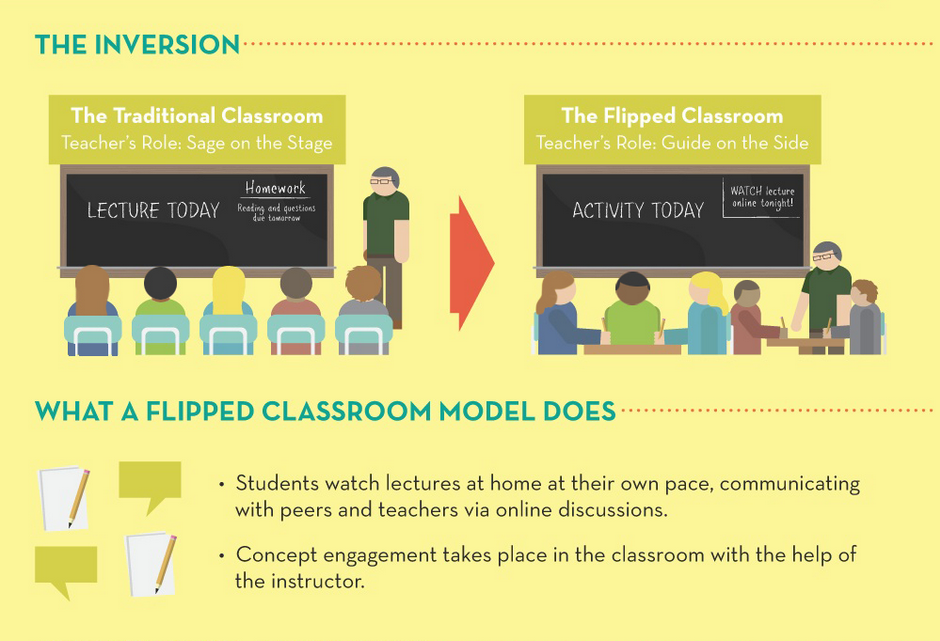
\includegraphics[width=\linewidth]{Imagens/flipped_classroom.png}
    \caption{Invers\~{a}o nos padr\~{o}es de ensino sugerida pelo modelo flipped classroom}
\end{figure}

%%%%%%%%%%%%%%%%%%%%%%%%%%%%%%%%%%%%%%%%%%%%%%%%%%%%%%%%%%%%%%%%%%%%%%%%%%%%%%%%
% Proposta %%%%%%%%%%%%%%%%%%%%%%%%%%%%%%%%%%%%%%%%%%%%%%%%%%%%%%%%%%%%%%%%%%%%%
%%%%%%%%%%%%%%%%%%%%%%%%%%%%%%%%%%%%%%%%%%%%%%%%%%%%%%%%%%%%%%%%%%%%%%%%%%%%%%%%

\chapter{Proposta}

O presente trabalho tem como objetivo desenvolver uma ferramenta, de cunho acad\^{e}mico
e opensource, que auxilie o ensino de banco de dados. O escopo do projeto abranger\'{a} o ensino
da linguagem SQL, atrav\'{e}s da disponibiliza\c{c}\~{a}o de exerc\'{i}cios online e f\'{o}rum para discuss\~{a}o dos
mesmos ou de assuntos referentes \`{a} disciplina. Al\'{e}m disso, todas as listas de exerc\'{i}cios contidas
no site ser\~{a}o, em um primeiro momento, as mesmas oferecidas na disciplina de Banco de Dados
da PUC--Rio (INF 1383).

Atualmente, os alunos da disciplina podem resolver os exerc\'{i}cios propostos em algumas
aulas pr\'{a}ticas, durante hor\'{a}rio de aula, ou utilizar um programa desktop que se conecta ao
servidor da disciplina com o \textbf{SGBD} \cite{ElmasriNavathe05} j\'{a} configurado. 
Os exerc\'{i}cios est\~{a}o vinculados, na maioria das vezes, a um ou mais esquemas contidos no SGBD 
em quest\~{a}o. Dessa forma, os alunos acessam um mesmo esquema para tentar solucionar determinada quest\~{a}o.
Quando trata-se de uma lista de exerc\'{i}cios que envolve puramente o comando \textbf{SELECT}, n\~{a}o h\'{a}
maiores problemas quanto ao esquema compartilhado.
Por\'{e}m, quando h\'{a} comandos \textbf{DML}\cite{ElmasriNavathe05} do tipo \textbf{INSERT}, \textbf{UPDATE} ou
\textbf{DELETE}, ou comandos \textbf{DDL}\cite{ElmasriNavathe05} envolvidos na resolu\c{c}\~{a}o da lista, pode-se
gerar uma indisponibiliza\c{c}\~{a}o moment\^{a}nea, caso um comando seja executado de forma incorreta.

Sendo assim, duas das principais caracter\'{i}sticas do sistema proposto ser\~{a}o a utiliza\c{c}\~{a}o de
esquemas distintos por alunos a cada quest\~{a}o e a possibilidade de voltar em uma determinada
modifica\c{c}\~{a}o feita anteriormente no esquema. Logo, al\'{e}m de ter liberdade de executar qualquer
comando na base, sabendo que n\~{a}o interferir\'{a} os demais alunos, o aluno poder\'{a} voltar em um
estado anterior da base quando bem entender.

%%%%%%%%%%%%%%%%%%%%%%%%%%%%%%%%%%%%%%%%%%%%%%%%%%%%%%%%%%%%%%%%%%%%%%%%%%%%%%%%
% Análise SWOT %%%%%%%%%%%%%%%%%%%%%%%%%%%%%%%%%%%%%%%%%%%%%%%%%%%%%%%%%%%%%%%%%
%%%%%%%%%%%%%%%%%%%%%%%%%%%%%%%%%%%%%%%%%%%%%%%%%%%%%%%%%%%%%%%%%%%%%%%%%%%%%%%%

\section{Avalia\c{c}\~{a}o do Sistema perante os Concorrentes -- An\'{a}lise SWOT}

A \textbf{An\'{a}lise SWOT} \cite{Fine09} \'{e} um sistema simples para posicionar ou verificar a
posi\c{c}\~{a}o estrat\'{e}gica da empresa no ambiente em quest\~{a}o. O termo SWOT \'{e} uma sigla
oriunda dos termos ingleses Strenghts (Forças), Weaknesses (Fraquezas), Opportunities (Oportunidades)
e Threats (Ameaças).

-- Strengths (forças) - vantagens internas da empresa em relação às concorrentes. Ex.:
qualidade do produto oferecido, bom serviço prestado ao cliente, solidez financeira, etc.

-- Weaknesses (fraquezas) - desvantagens internas da empresa em relação às concorrentes.
Ex.: altos custos de produção, má imagem, instalações desadequadas, marca fraca, etc.;

-- Opportunities (oportunidades) – aspectos externos positivos que podem potenciar a
vantagem competitiva da empresa. Ex.: mudanças nos gostos dos clientes, falência de
empresa concorrente, etc.;

-- Threats (ameaças) - aspectos externos negativos que podem por em risco a vantagem
competitiva da empresa. Ex.: novos competidores, perda de trabalhadores fundamentais,
etc.

\begin{figure}[H]
    \centering
    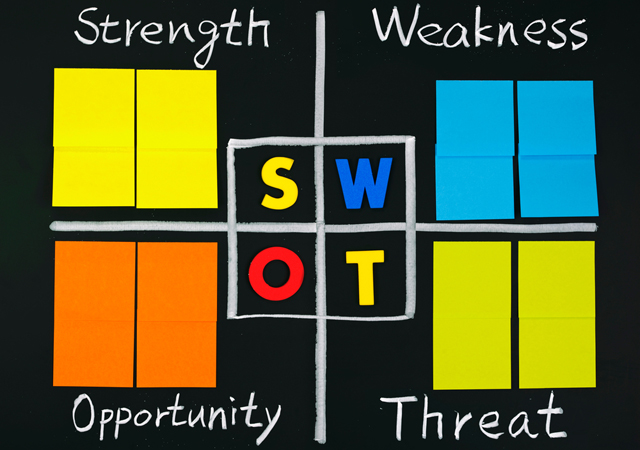
\includegraphics[width=\linewidth]{Imagens/swot.jpg}
    \caption{Ilustração que demonstra todos os critérios utilizados na Análise SWOT}
\end{figure}

Segue a seguir a an\'{a}lise do projeto perante os concorrentes:

\begin{table}[H]
    \resizebox{\linewidth}{!}{
    \begin{tabular}{|l|}
    \hline
    \textbf{Forças}                                                                              \\ \hline
    Sistema focado no aprendizado de apenas uma disciplina                                       \\ \hline
    Ferramenta opensource e gratuita                                                             \\ \hline
    Apenas o Gradiance possui curso específico para aprendizado de Banco de Dados                \\ \hline
    Listas de exercícios extensa e aplicada por anos com sucesso na disciplina de Banco de Dados \\ \hline
    Exercícios com feedback instantâneo aos alunos                                               \\ \hline
    \textbf{Fraquezas}                                                                           \\ \hline
    Publico alvo restrito a alunos da PUC-Rio                                                    \\ \hline
    Novo entrante no mercado                                                                     \\ \hline
    Não possui reconhecimento internacional como cursos do Edx                                   \\ \hline
    \textbf{Oportunidades}                                                                       \\ \hline
    Ferramenta facilmente acessível pelos alunos e professores                                   \\ \hline
    Apenas o Gradiance possui curso específico para aprendizado de Banco de Dados                \\ \hline
    Maior independencia no aprendizado do aluno (aprender fora da sala de aula)                  \\ \hline
    Gerar maior interesse nos alunos, pois aprende-se fazendo (aprendizado no prática)           \\ \hline
    Conceito de Flipped Learning ainda pouco desenvolvido no Brasil                              \\ \hline
    \textbf{Ameaças}                                                                             \\ \hline
    Desinteresse dos alunos pelo aprendizado de Banco de Dados                                   \\ \hline
    Desinteresse dos alunos pela utilização da ferramenta                                        \\ \hline
    \end{tabular}
    }
\end{table}

%%%%%%%%%%%%%%%%%%%%%%%%%%%%%%%%%%%%%%%%%%%%%%%%%%%%%%%%%%%%%%%%%%%%%%%%%%%%%%%%
% Requisitos %%%%%%%%%%%%%%%%%%%%%%%%%%%%%%%%%%%%%%%%%%%%%%%%%%%%%%%%%%%%%%%%%%%
%%%%%%%%%%%%%%%%%%%%%%%%%%%%%%%%%%%%%%%%%%%%%%%%%%%%%%%%%%%%%%%%%%%%%%%%%%%%%%%%

\section{Requisitos}

\subsection{Escopo}

A lista a seguir se refere \`{a} elicita\c{c}\~{a}o de requisitos \cite{Leite03} referentes a uma plataforma de ensino online.
A mesma conter\'{a} tanto \textbf{requisitos funcionais} quanto \textbf{requisitos n\~{a}o funcionais}.

\subsection{P\'{u}blico Alvo}

Em um primeiro momento, a plataforma em quest\~{a}o se destina a estudantes da Pontif\'{i}cia Universidade
Cat\'{o}lica do Rio de Janeiro que estejam cursando a disciplina de Banco de Dados. Em um futuro pr\'{o}ximo, 
deseja--se disponibilizar o projeto a diversos cursos.

\subsection{Requisitos N\~{a}o Funcionais}

[R1] Realiza\c{c}\~{a}o de um estudo sobre os principais concorrentes da plataforma, utilizando a An\'{a}lise SWOT.

[R2] Documenta\c{c}\~{a}o do sistema utilizando pr\'{a}ticas conhecidas: Modelagem Conceitual, Modelagem L\'{o}gica,
Modelagem F\'{i}sica, Casos de Uso e Diagrama de Classes.

[R3] Utiliza\c{c}\~{a}o de documenta\c{c}\~{a}o interna do c\'{o}digo, com o intuito de facilitar a modifica\c{c}\~{a}o da 
plataforma no futuro.

[R4] Gerenciamento de vers\~{o}es do c\'{o}digo utilizando a ferramenta Git com a plataforma GitHub.

[R5] Cria\c{c}\~{a}o de Mockups das telas do sistema.

\subsection{Requisitos Funcionais}

[R6] A plataforma de ensino ter\'{a} a funcionalidade de controle de acesso, existindo dois n\'{i}veis de usu\'{a}rio:
Aluno e Professor.

\textbf{Funcionalidades Professor:}

[R7] Controle dos alunos que possuem acesso a ferramenta.

[R8] M\'{o}dulo de edi\c{c}\~{a}o dos exerc\'{i}cios e quest\~{o}es.

[R9] Carga dos esquemas utilizados nos exerc\'{i}cios.

[R10] Monitoramento da evolu\c{c}\~{a}o dos alunos.

[R11] Permiss\~{a}o para cancelar uma thread inadequada no f\'{o}rum.

\textbf{Funcionalidades Aluno:}

[R12] Utiliza\c{c}\~{a}o de uma inst\^{a}ncia pr\'{o}pria a cada exerc\'{i}cio.

[R13] Possibilidade de compartilhar com seus colegas de turma suas inst\^{a}ncias.

[R14] Utiliza\c{c}\~{a}o de f\'{o}rum como forma de sanar d\'{u}vidas dos exerc\'{i}cios e auxiliar os outros alunos.

[R15] Resolu\c{c}\~{a}o dos exerc\'{i}cios com corre\c{c}\~{a}o dos mesmos em tempo real.

[R16] Possibilidade de fazer upload de foto para facilitar a identifica\c{c}\~{a}o do aluno.

[R17] Possibilidade de compartilhar as quest\~{o}es em redes sociais (Facebook, Google+ e Twiter).

%%%%%%%%%%%%%%%%%%%%%%%%%%%%%%%%%%%%%%%%%%%%%%%%%%%%%%%%%%%%%%%%%%%%%%%%%%%%%%%%
% Projeto %%%%%%%%%%%%%%%%%%%%%%%%%%%%%%%%%%%%%%%%%%%%%%%%%%%%%%%%%%%%%%%%%%%%%%
%%%%%%%%%%%%%%%%%%%%%%%%%%%%%%%%%%%%%%%%%%%%%%%%%%%%%%%%%%%%%%%%%%%%%%%%%%%%%%%%

\chapter{Projeto}

Neste t\'{o}pico ser\~{a}o expostos todas as abstra\c{c}\~{o}es de projeto realizadas em ordem
cronol\'{o}gica. Essa evolu\c{c}\~{a}o sequencial permitiu um melhor entendimento do problema e,
consequentemente, uma clara defini\c{c}\~{a}o de escopo.

Iniciando pela Modelagem Conceitual [3.1], com a utiliza\c{c}\~{a}o do modelo entidade
relacionamento, foi poss\'{i}vel obter uma alta abstra\c{c}\~{a}o da plataforma, assim como um melhor
entendimento das regras de neg\'{o}cios envolvidas \cite{Heuser09}. Logo ap\'{o}s foram feitas as modelagens L\'{o}gica
[3.2] e F\'{i}sica [3.3]. Na l\'{o}gica, explicitamos a estrutura a ser utilizada para persist\^{e}ncia dos dados,
que no caso fora em tabelas, e os tipos de dados de cada atributo. J\'{a} na f\'{i}sica, foi definido o
SGBD utilizado, que no caso fora o \textbf{PostgreSQL 9.1}, e definidas os comandos SQL do tipo DDL
para criação das tabelas, chaves primárias e estrangeiras, triggers, constraints, entre outros.

\begin{figure}[H]
    \centering
    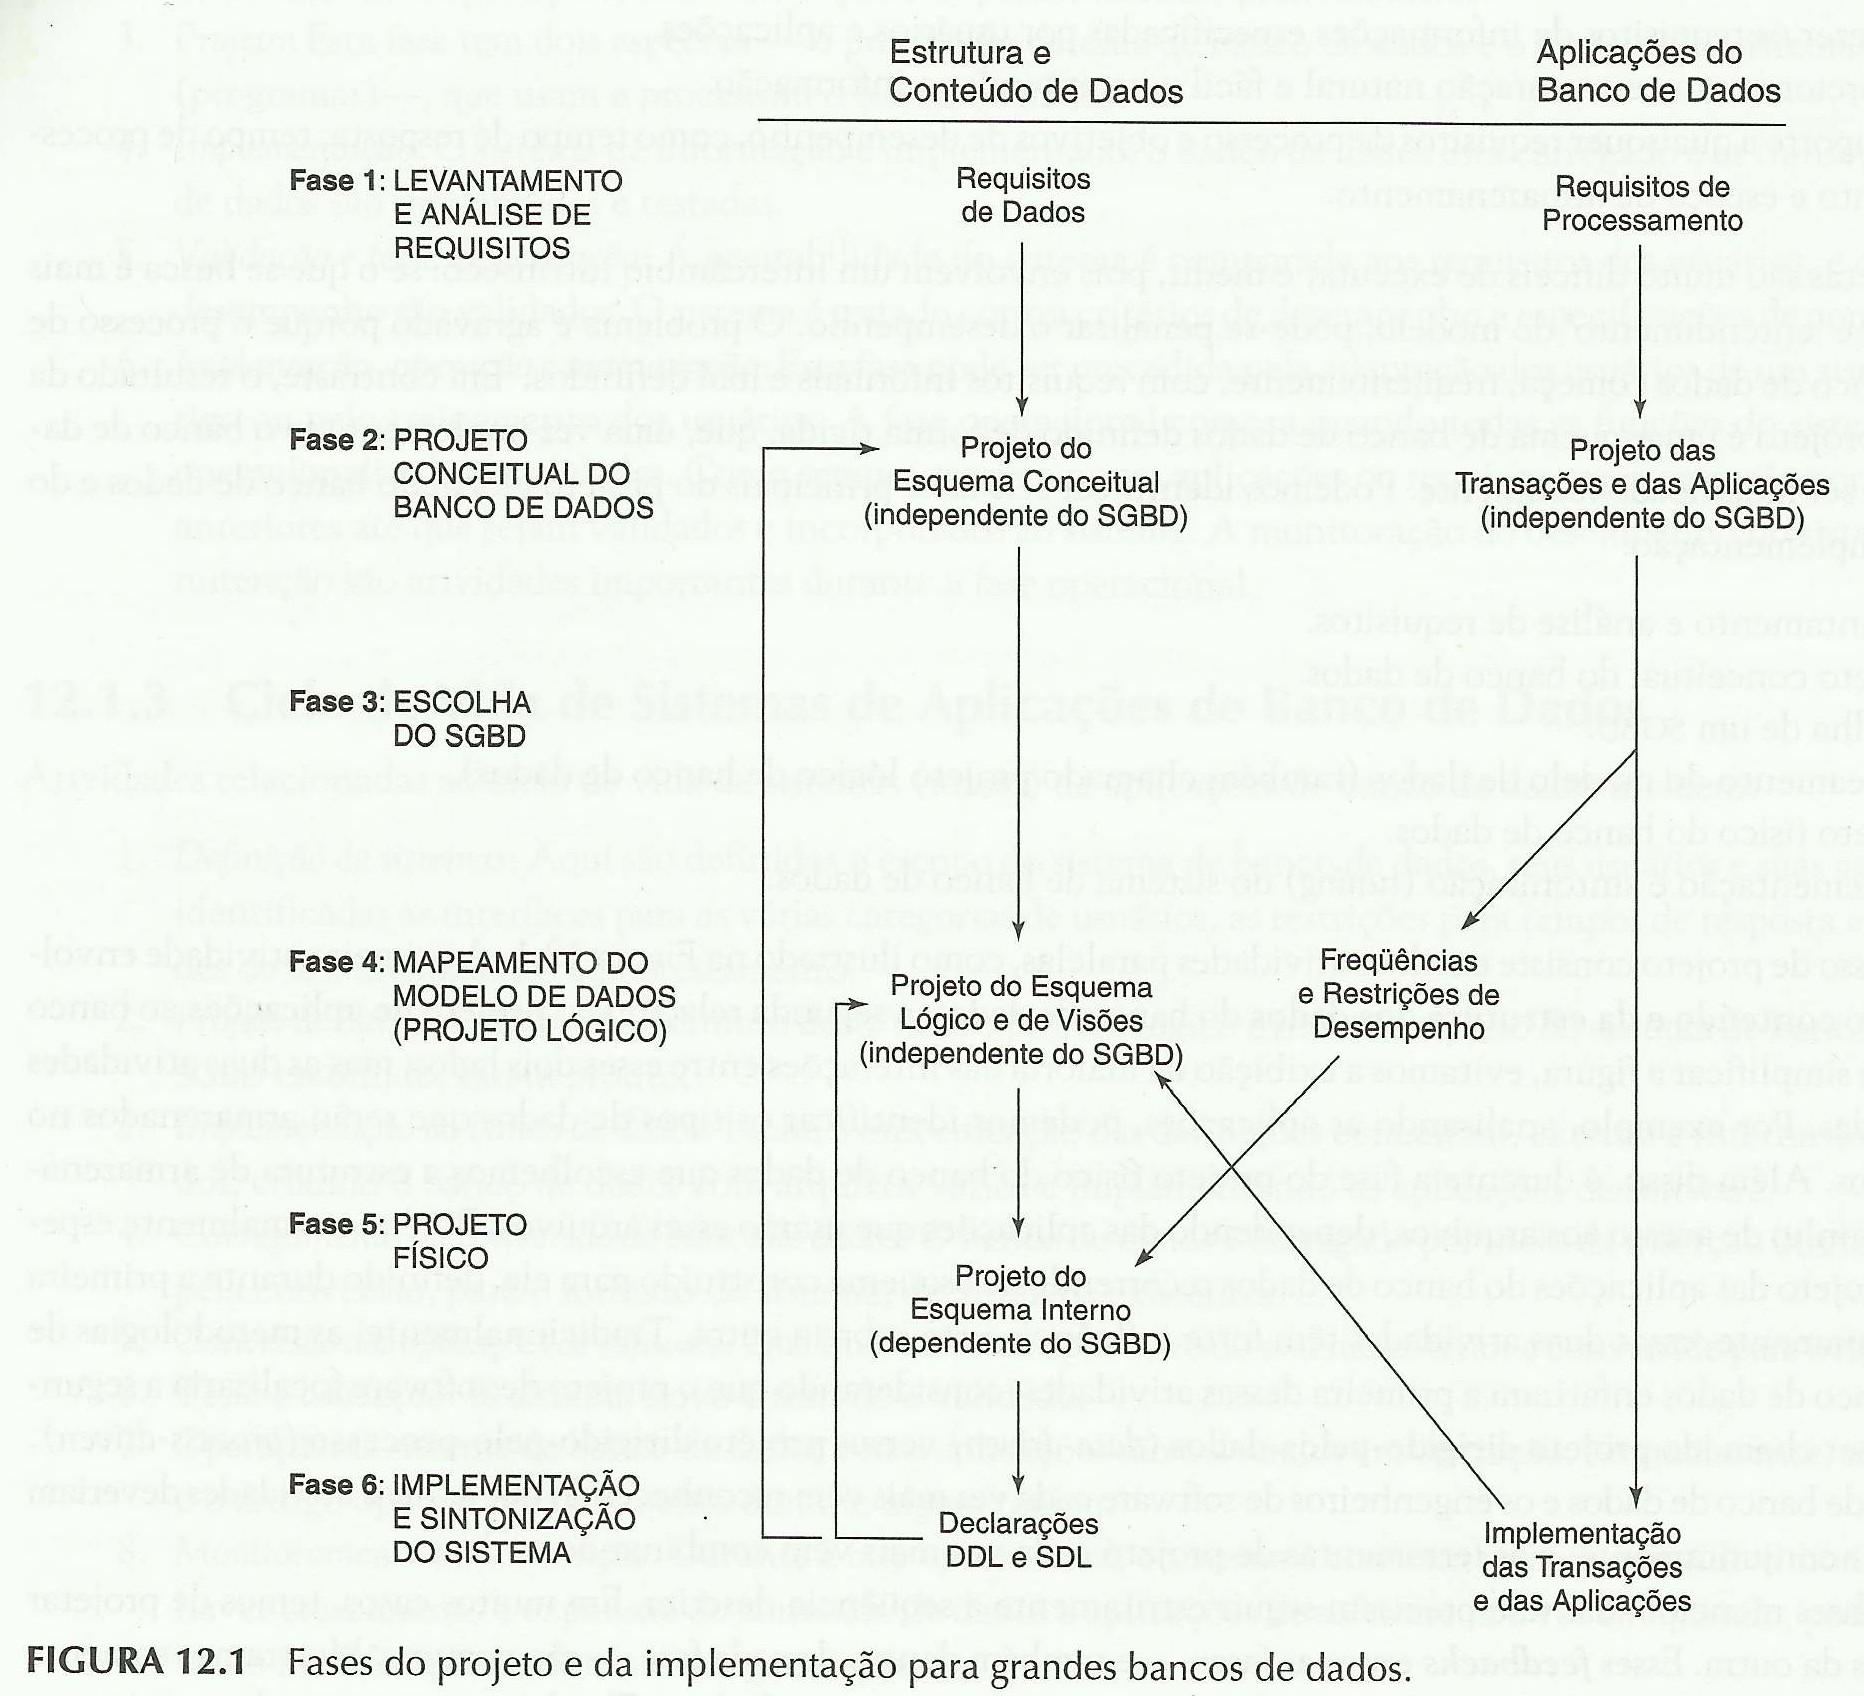
\includegraphics[width=\linewidth]{Imagens/fases_projeto_banco_dados.jpg}
    \caption{Fases do projeto e da implementação de banco de dados sugerida no livro 
	     \textbf{'Sistemas de Banco de Dados', 4a edição, Elsmari e Navathe}}
\end{figure}

Ap\'{o}s terminadas as abstra\c{c}\~{o}es referentes ao armazenamento dos dados, partimos para a
defini\c{c}\~{a}o da intera\c{c}\~{a}o entre os usu\'{a}rios envolvidos e o sistema, atrav\'{e}s dos Casos de Uso [3.4]
\cite{Larman04}, e para a defini\c{c}\~{a}o da arquitetura a ser utilizada no desenvolvimento da plataforma, atrav\'{e}s do
Diagrama de Classes [3.5].

%%%%%%%%%%%%%%%%%%%%%%%%%%%%%%%%%%%%%%%%%%%%%%%%%%%%%%%%%%%%%%%%%%%%%%%%%%%%%%%%
% Modelagem Conceitual %%%%%%%%%%%%%%%%%%%%%%%%%%%%%%%%%%%%%%%%%%%%%%%%%%%%%%%%%
%%%%%%%%%%%%%%%%%%%%%%%%%%%%%%%%%%%%%%%%%%%%%%%%%%%%%%%%%%%%%%%%%%%%%%%%%%%%%%%%

\section{Modelagem Conceitual}

Nesta se\c{c}\~{a}o vamos mostrar a evolu\c{c}\~{a}o da concep\c{c}\~{a}o do projeto atrav\'{e}s das tr\^{e}s vers\~{o}es
elaboradas com o uso do diagrama entidade relacionamento.

\begin{figure}[H]
    \centering
    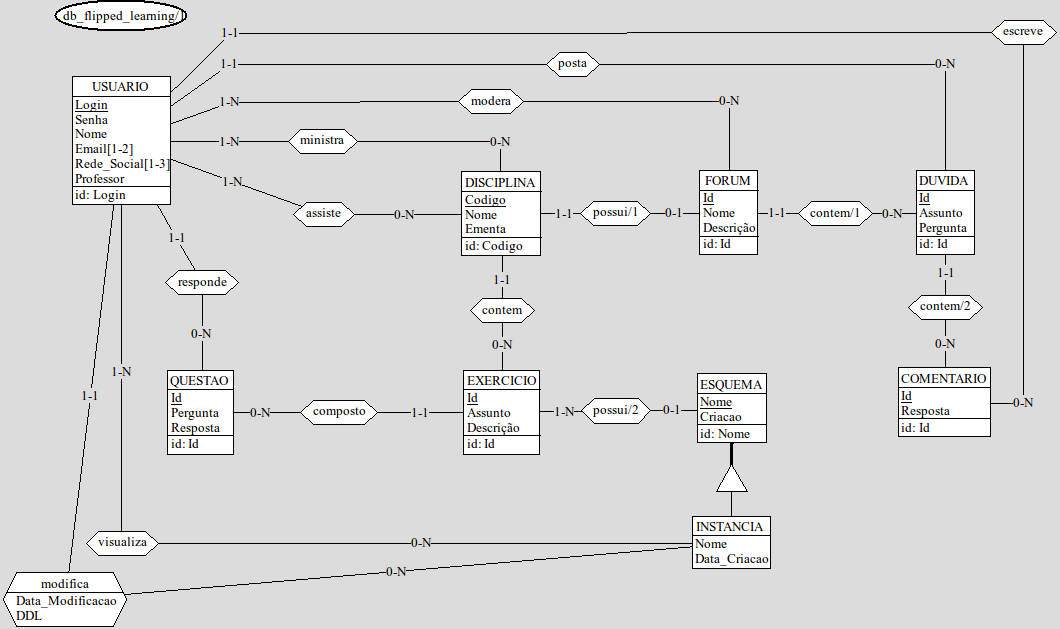
\includegraphics[width=\linewidth]{Imagens/ModelagemConceitual_v1_0.png}
    \caption{Primeira versão da Modelagem Conceitual}
\end{figure}

A entidade usu\'{a}rio serve como representa\c{c}\~{a}o tanto para aluno, quanto para professor.
Como n\~{a}o foram encontrados atributos \'{u}nicos que fossem capazes de diferenciar as poss\'{i}veis
entidades aluno e professor, n\~{a}o houve necessidade da utiliza\c{c}\~{a}o de heran\c{c}a (tamb\'{e}m chamado
de “IS-A”). No caso, haveria a possibilidade de aluno e professor herdarem caracter\'{i}sticas da
entidade usu\'{a}rio. Para a diferencia\c{c}\~{a}o do papel, aluno ou professor, fora utilizado o atributo
'professor' (depois ser\'{a} poss\'{i}vel perceber que o mesmo deixou de ser utilizado, por n\~{a}o se fazer
necess\'{a}ria a distin\c{c}\~{a}o de pap\'{e}is nesse n\'{i}vel de abstra\c{c}\~{a}o do modelo).

Cada exerc\'{i}cio proposto poder\'{a}, ou n\~{a}o, ser vinculado, a um esquema. Dessa forma, o
sistema foi idealizado para permitir n\~{a}o s\'{o} quest\~{o}es relacionadas a SQL, mas a qualquer tema
abordado na disciplina Banco de Dados. Como caracter\'{i}sticas, a entidade esquema possui um
nome, como identificador, e um campo destinado a seu DDL de cria\c{c}\~{a}o, chamado cria\c{c}\~{a}o.
Quando um aluno inicia um novo exerc\'{i}cio e caso o mesmo seja vinculado a um esquema
para ser respondido, \'{e} criado uma inst\^{a}ncia. A inst\^{a}ncia nada mais \'{e} do que uma c\'{o}pia, em seu
estado inicial, do esquema associado ao exerc\'{i}cio. Essa escolha foi tomada a fim de dar maior
liberdade na utiliza\c{c}\~{a}o da base por parte dos alunos. \'{E} comum, em outras plataformas, a
exist\^{e}ncia de bases compartilhadas para resolu\c{c}\~{a}o dos exerc\'{i}cios em SQL. Por\'{e}m, acredita-se
que essa pr\'{a}tica inibe o aluno (como mencionado em se\c{c}\~{a}o anterior), que passa a ter medo de
errar e prejudicar a turma.

Ainda em rela\c{c}\~{a}o a inst\^{a}ncia, foi dada a liberdade para que o aluno possa compartilh\'{a}-la
com seus colegas de turma. O mesmo fica expl\'{i}cito ao analisarmos a cardinalidade do
relacionamento “visualiza”, entre as entidades usu\'{a}rio e inst\^{a}ncia. J\'{a} em rela\c{c}\~{a}o a a\c{c}\~{a}o de
“modifica\c{c}\~{a}o” da inst\^{a}ncia, apenas o usu\'{a}rio dono na mesma poder\'{a} realiz\'{a}-la.
Para haver maior intera\c{c}\~{a}o dos usu\'{a}rio com a plataforma, foi possibilitada a cria\c{c}\~{a}o uma
\'{a}rea de f\'{o}rum por disciplina. E o usu\'{a}rio com o papel de professor seria o moderador, j\'{a} os alunos
participariam com d\'{u}vidas e coment\'{a}rios relacionados a mat\'{e}ria dada.

A caracter\'{i}stica preponderante desta vers\~{a}o era fazer uma plataforma que englobasse
diversas disciplinas. Por\'{e}m, conforme foi sendo definido o escopo, p\^{o}de-se observar que um fator
de diferencia\c{c}\~{a}o perante os demais sistemas seria o foco no tema banco de dados. Essa escolha
provocou uma melhor visualiza\c{c}\~{a}o da solu\c{c}\~{a}o, que pode ser percebido nas duas seguintes
vers\~{o}es.

\begin{figure}[H]
    \centering
    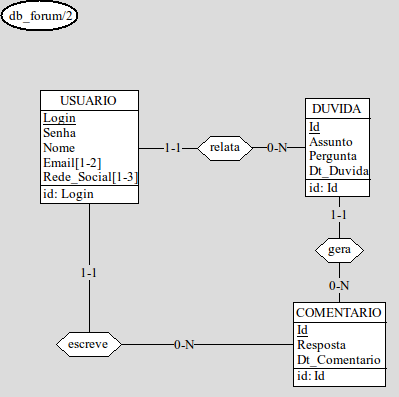
\includegraphics[width=\linewidth]{Imagens/ModelagemConceitual_forum_v1_1.png}
    \caption{Segunda vers\~{a}o da Modelagem Conceitual; solu\c{c}\~{a}o focada no f\'{o}rum}
\end{figure}

\begin{figure}[H]
    \centering
    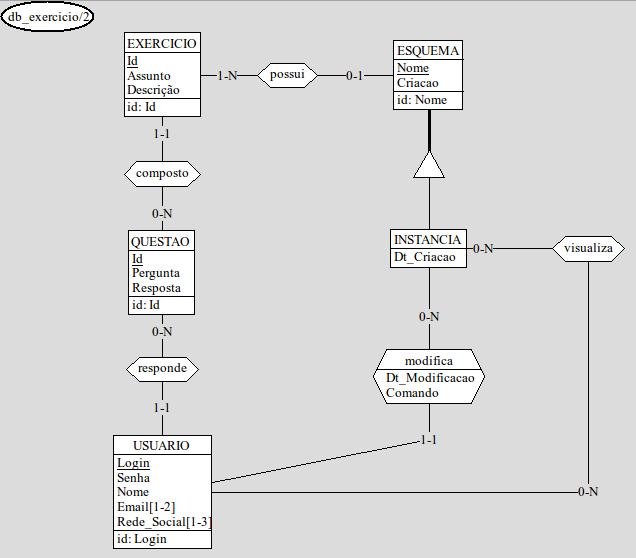
\includegraphics[width=\linewidth]{Imagens/ModelagemConceitual_exercicio_v1_1.png}
    \caption{Segunda vers\~{a}o da Modelagem Conceitual; solu\c{c}\~{a}o focada nos exerc\'{i}cios}
\end{figure}

Tendo em vista que a primeira vers\~{a}o havia ficado muito confusa, foi decidido particionar a
solu\c{c}\~{a}o em dois sistemas distintos: f\'{o}rum e exerc\'{i}cio. Dessa forma, houve uma simplifica\c{c}\~{a}o do
problema, al\'{e}m da melhor compreens\~{a}o do mesmo, que certamente ajudar\'{a} nas pr\'{o}ximas etapas
do projeto.

Alguns aspectos relevantes precisam ser ressaltados. A modelagem referente ao f\'{o}rum
apresenta um caminho fechado, o que deve ser evitado. Por\'{e}m, um caminho fechado n\~{a}o
necessariamente \'{e} um ciclo. J\'{a} um ciclo \'{e}, necessariamente, um caminho fechado. Assim sendo,
devemos observar o sentido do relacionamento. E como um usu\'{a}rio, no papel de aluno, relata a
d\'{u}vida e um usu\'{a}rio, no papel de aluno ou professor, escreve o coment\'{a}rio, podemos perceber
que n\~{a}o h\'{a} gera\c{c}\~{a}o de ciclo.

Mesmo com a evolu\c{c}\~{a}o entre as vers\~{o}es, alguns requisitos do sistema n\~{a}o foram
contemplados, tais como os moderadores do f\'{o}rum e a persist\^{e}ncia das respostas dos alunos \`{a}s
quest\~{o}es dos exerc\'{i}cios. Al\'{e}m disso uma d\'{u}vida se fez presente: ser\'{a} mesmo que uma inst\^{a}ncia
\'{e} um esquema?

\begin{figure}[H]
    \centering
    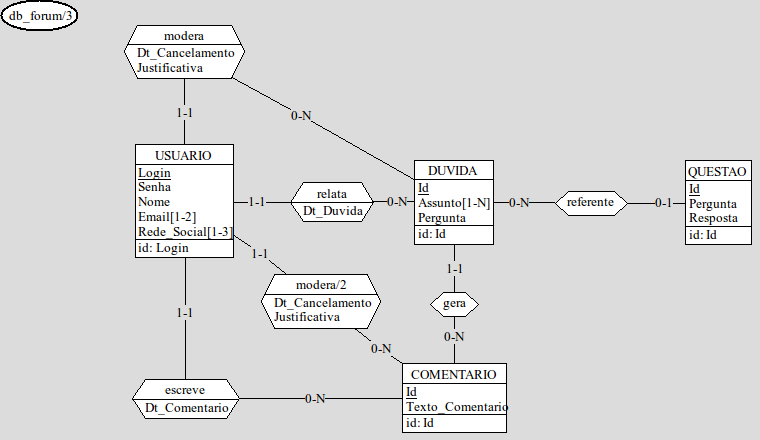
\includegraphics[width=\linewidth]{Imagens/ModelagemConceitual_forum_v2_0.png}
    \caption{Terceira vers\~{a}o da Modelagem Conceitual; solu\c{c}\~{a}o focada no f\'{o}rum}
\end{figure}

\begin{figure}[H]
    \centering
    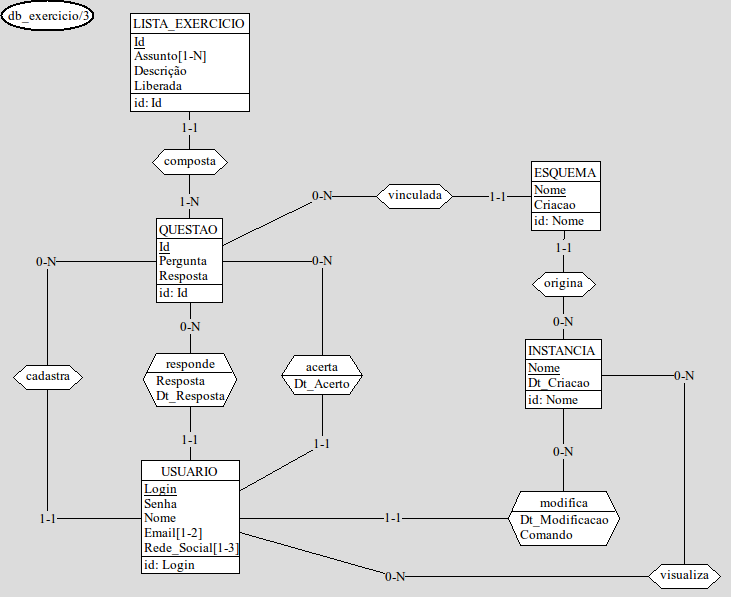
\includegraphics[width=\linewidth]{Imagens/ModelagemConceitual_exercicio_v2_0.png}
    \caption{Terceira vers\~{a}o da Modelagem Conceitual; solu\c{c}\~{a}o focada nos exerc\'{i}cios}
\end{figure}

Com rela\c{c}\~{a}o a modelagem referente ao f\'{o}rum, podemos perceber a adi\c{c}\~{a}o das datas no
relacionamento “relatar” e “escrever”, ao inv\'{e}s de estarem presentes nas entidades d\'{u}vida e
coment\'{a}rio, respectivamente. Tamb\'{e}m foram adicionadas as a\c{c}\~{o}es de “modera\c{c}\~{a}o” do f\'{o}rum,
que anteriormente n\~{a}o foram contempladas. Em ambas um campo de 'justificativa' fora inserido,
para permitir que o moderador possa explicar os motivos de um poss\'{i}vel cancelamento de d\'{u}vida
ou coment\'{a}rio.

Al\'{e}m disso, perceba que a entidade d\'{u}vida agora pode, ou n\~{a}o, estar relacionada com a
entidade quest\~{a}o. Dessa maneira, foi possibilitada a inser\c{c}\~{a}o de d\'{u}vidas n\~{a}o somente aos
exerc\'{i}cios contidos na plataforma, mas como d\'{u}vidas te\'{o}ricas, que tenham sido abordadas na
disciplina, ou exerc\'{i}cios de fontes externas, por exemplo de outras faculdades.

Com rela\c{c}\~{a}o a modelagem referente aos exerc\'{i}cios, as entidades esquema e inst\^{a}ncia
deixarem de ser, respectivamente, superclasse e subclasse uma da outra. Logo, houve uma
substitui\c{c}\~{a}o da representa\c{c}\~{a}o de heran\c{c}a por uma de relacionamento, com a a\c{c}\~{a}o “originar”.

Outro ponto importante \'{e} a persist\^{e}ncia das respostas dos usu\'{a}rios \`{a}s quest\~{o}es. Ser\~{a}o
armazenadas tanto as respostas corretas como as incorretas. Houve a op\c{c}\~{a}o de representar a
a\c{c}\~{a}o de “acerto” separado da a\c{c}\~{a}o de “resposta”. Logo, deve-se tomar cuidado para manter a
restri\c{c}\~{a}o de integridade sem\^{a}ntica nesse caso, j\'{a} que devemos identificar quais das respostas do
usu\'{a}rio fora a correta.

Perceba que o relacionamento da a\c{c}\~{a}o “v\'{i}nculo” era entre as entidades exerc\'{i}cio e
esquema. Todavia, uma lista de exerc\'{i}cios pode conter quest\~{o}es referentes a diferentes
esquemas. Assim sendo, a entidade quest\~{a}o passa a estar vinculada a um determinado esquema.

%%%%%%%%%%%%%%%%%%%%%%%%%%%%%%%%%%%%%%%%%%%%%%%%%%%%%%%%%%%%%%%%%%%%%%%%%%%%%%%%
% Modelagem Lógica %%%%%%%%%%%%%%%%%%%%%%%%%%%%%%%%%%%%%%%%%%%%%%%%%%%%%%%%%%%%%
%%%%%%%%%%%%%%%%%%%%%%%%%%%%%%%%%%%%%%%%%%%%%%%%%%%%%%%%%%%%%%%%%%%%%%%%%%%%%%%%

\section{Modelagem L\'{o}gica}

Nesta fase, o mapeamento ainda n\~{a}o considera nenhuma caracter\'{i}stica espec\'{i}fica ou
casos especiais que se aplicam \`{a} implementa\c{c}\~{a}o do modelo de dados do SGBD. Ou seja, tudo
que for relatado pode ser aplicado a qualquer escolha de SGBD na pr\'{o}xima etapa.

Dessa forma, foram listadas todas as tabelas com suas chaves prim\'{a}rias e estrangeiras
identificadas, atributos e tipos de dados. Al\'{e}m disso, foram identificados os campos: Entidade,
Atributo e Relacionamento. Com esses campos, foi poss\'{i}vel realizar o rastro entre a Modelagem
Conceitual e a Modelagem L\'{o}gica.

%%%%%%%%%%%%%%%%%%%%%%%%%%%%%%%%%%%%%%%%%%%%%%%%%%%%%%%%%%%%%%%%%%%%%%%%%%%%%%%%
% Tabela Exercícios Parte 1 %%%%%%%%%%%%%%%%%%%%%%%%%%%%%%%%%%%%%%%%%%%%%%%%%%%%
%%%%%%%%%%%%%%%%%%%%%%%%%%%%%%%%%%%%%%%%%%%%%%%%%%%%%%%%%%%%%%%%%%%%%%%%%%%%%%%%

\begin{table}[H]
    \resizebox{\linewidth}{!}{
    \begin{tabular}{|l|l|l|l|l|l|l|l|}
    \hline
    \multicolumn{8}{|l|}{lista\_exercicio} \\ \hline
    ID                      & Atributos      & Tipo                 & Tamanho/Formato & Extra            & Entidade        & Atributo       & Relacionamento  \\ \hline
    1                       & id             & inteiro              & -               & auto incremental & LISTA\_EXERCICIO & Id             & -               \\ \hline
    2                       & id\_assunto    & inteiro              & -               & -                & LISTA\_EXERCICIO & Assunto[1-N]   & -               \\ \hline
    3                       & descricao      & cadeia de caracteres & 1024            & -                & LISTA\_EXERCICIO & Descrição      & -               \\ \hline
    4                       & dt\_liberada   & data                 & dd-mm-aaaa      & -                & LISTA\_EXERCICIO & Liberada       & -               \\ \hline
    \multicolumn{8}{|l|}{questao} \\ \hline
    ID                      & Atributos      & Tipo                 & Tamanho/Formato & Extra            & Entidade        & Atributo       & Relacionamento  \\ \hline
    1                       & id             & inteiro              & -               & auto incremental & QUESTAO         & Id             & -               \\ \hline
    2                       & id\_exercicio  & inteiro              & -               & -                & LISTA\_EXERCICIO & Id             & composta        \\ \hline
    3                       & login\_usuario & cadeia de caracteres & 20              & -                & USUARIO         & Login          & cadastra        \\ \hline
    4                       & nome\_esquema  & cadeia de caracteres & 50              & -                & ESQUEMA         & Nome           & -               \\ \hline
    5                       & pergunta       & cadeia de caracteres & 1024            & -                & QUESTAO         & Pergunta       & -               \\ \hline
    6                       & resposta       & cadeia de caracteres & 1024            & -                & QUESTAO         & Resposta       & -               \\ \hline
    \multicolumn{8}{|l|}{usuario} \\ \hline
    ID                      & Atributos      & Tipo                 & Tamanho/Formato & Extra            & Entidade        & Atributo       & Relacionamento  \\ \hline
    1                       & login          & cadeia de caracteres & 20              & -                & USUARIO         & Login          & -               \\ \hline
    2                       & senha          & cadeia de caracteres & 15              & -                & USUARIO         & Senha          & -               \\ \hline
    3                       & nome           & cadeia de caracteres & 100             & -                & USUARIO         & Nome           & -               \\ \hline
    4                       & e-mail         & cadeia de caracteres & 100             & -                & USUARIO         & Email          & -               \\ \hline
    5                       & professor      & booleano             & 1               & -                & -               & -              & -               \\ \hline
    \multicolumn{8}{|l|}{resposta} \\ \hline
    ID                      & Atributos      & Tipo                 & Tamanho/Formato & Extra            & Entidade        & Atributo       & Relacionamento  \\ \hline
    1                       & id             & inteiro              & -               & auto incremental & -               & -              & -               \\ \hline
    2                       & id\_questao    & inteiro              & -               & -                & QUESTAO         & Id             & -               \\ \hline
    3                       & login\_usuario & cadeia de caracteres & 20              & -                & USUARIO         & Login          & -               \\ \hline
    4                       & dt\_resposta   & data                 & dd-mm-aaaa      & -                & -               & Dt\_Resposta   & responde        \\ \hline
    5                       & dt\_acerto     & data                 & dd-mm-aaaa      & -                & -               & Dt\_Acerto     & acerta          \\ \hline
    6                       & resposta       & cadeia de caracteres & 1024            & -                & -               & Resposta       & responde        \\ \hline
    \multicolumn{8}{|l|}{esquema} \\ \hline
    ID                      & Atributos      & Tipo                 & Tamanho/Formato & Extra            & Entidade        & Atributo       & Relacionamento  \\ \hline
    1                       & nome           & cadeia de caracteres & 50              & -                & ESQUEMA         & Nome           & -               \\ \hline
    2                       & criacao        & cadeia de caracteres & 4096            & -                & ESQUEMA         & Criacao        & -               \\ \hline
    \multicolumn{8}{|l|}{instancia} \\ \hline
    ID                      & Atributos      & Tipo                 & Tamanho/Formato & Extra            & Entidade        & Atributo       & Relacionamento  \\ \hline
    1                       & nome           & cadeia de caracteres & 50              & -                & INSTANCIA       & Nome           & -               \\ \hline
    2                       & nome\_esquema  & cadeia de caracteres & 50              & -                & ESQUEMA         & Nome           & -               \\ \hline
    3                       & login\_usuario & cadeia de caracteres & 20              & -                & USUARIO         & Login          & -               \\ \hline
    4                       & dt\_criacao    & data                 & dd-mm-aaaa      & -                & INSTANCIA       & Dt\_Criacao    & -               \\ \hline
    \multicolumn{8}{|l|}{modificacao} \\ \hline
    ID                      & Atributos      & Tipo                 & Tamanho/Formato & Extra            & Entidade        & Atributo       & Relacionamento  \\ \hline
    1                       & id             & inteiro              & -               & auto incremental & -               & -              & -               \\ \hline
    2                       & nome\_instancia & cadeia de caracteres & 50              & -                & INSTANCIA       & Nome           & -               \\ \hline
    3                       & login\_usuario & cadeia de caracteres & 20              & -                & USUARIO         & Login          & -               \\ \hline
    4                       & dt\_modificacao & data                 & dd-mm-aaaa      & -                & -               & Dt\_Modificacao & modifica        \\ \hline
    5                       & comando        & cadeia de caracteres & 1024            & -                & -               & Comando        & modifica        \\ \hline
    \multicolumn{8}{|l|}{visualizacao} \\ \hline
    ID                      & Atributos      & Tipo                 & Tamanho/Formato & Extra            & Entidade        & Atributo       & Relacionamento  \\ \hline
    1                       & nome\_instancia & cadeia de caracteres & 50              & -                & INSTANCIA       & Nome           & -               \\ \hline
    2                       & login\_usuario & cadeia de caracteres & 20              & -                & USUARIO         & Login          & -               \\ \hline
    \multicolumn{8}{|l|}{assunto} \\ \hline
    ID                      & Atributos      & Tipo                 & Tamanho/Formato & Extra            & Entidade        & Atributo       & Relacionamento  \\ \hline
    1                       & id             & inteiro              & -               & auto incremental & LISTA\_EXERCICIO & Assunto[1-N]   & -               \\ \hline
    2                       & nome           & cadeia de caracteres & 100             & -                & LISTA\_EXERCICIO & Assunto[1-N]   & -               \\ \hline
    \multicolumn{8}{|l|}{assunto\_lista\_exercicio} \\ \hline
    ID                      & Atributos      & Tipo                 & Tamanho/Formato & Extra            & Entidade        & Atributo       & Relacionamento  \\ \hline
    1                       & id\_assunto    & inteiro              & -               & -                & LISTA\_EXERCICIO & Assunto[1-N]   & -               \\ \hline
    2                       & id\_exercicio  & inteiro              & -               & -                & LISTA\_EXERCICIO & Id             & -               \\ \hline
    \end{tabular}
    }
    \caption {Tabelas referentes a Lista de Exerc\'{i}cios (parte 1)}
\end{table}

%%%%%%%%%%%%%%%%%%%%%%%%%%%%%%%%%%%%%%%%%%%%%%%%%%%%%%%%%%%%%%%%%%%%%%%%%%%%%%%%
% Tabela Exercícios Parte 2 %%%%%%%%%%%%%%%%%%%%%%%%%%%%%%%%%%%%%%%%%%%%%%%%%%%%
%%%%%%%%%%%%%%%%%%%%%%%%%%%%%%%%%%%%%%%%%%%%%%%%%%%%%%%%%%%%%%%%%%%%%%%%%%%%%%%%

\begin{table}[H]
    \tiny
    \resizebox{\linewidth}{!}{
    \begin{tabular}{|l|l|}
    \hline
    \multicolumn{2}{|l|}{lista\_exercicio} \\ \hline
    ID                      & Observações                                                                                           \\ \hline
    1                       & Identificador da tupla.                                                                               \\ \hline
    2                       & Informa quais temas são abordados na lista de exercício.                                              \\ \hline
    3                       & Possível sugestões do professor de como resolver a lista, com sugestão de referências bibliográficas. \\ \hline
    4                       & Armazena em que dia a lista fora liberada aos alunos.                                                 \\ \hline
    \multicolumn{2}{|l|}{questao} \\ \hline
    ID                      & Observações                                                                                           \\ \hline
    1                       & Identificador da tupla.                                                                               \\ \hline
    2                       & Identifica a qual lista de exercício a questão está atrelada.                                         \\ \hline
    3                       & Identificação do usuário responsável pela criação da questão.                                         \\ \hline
    4                       & Identifica a qual esquema a questão pode estar vinculada.                                             \\ \hline
    5                       & Informa o enunciado da questão a ser respondida pelo aluno.                                           \\ \hline
    6                       & Trata-se do gabarito dado pelo professor.                                                             \\ \hline
    \multicolumn{2}{|l|}{usuario} \\ \hline
    ID                      & Observações                                                                                           \\ \hline
    1                       & Identificador da tupla, criado pelo usuário e faz parte da sua chave de acesso ao sistema.            \\ \hline
    2                       & Criado pelo usuário e faz parte da sua chave de acesso ao sistema.                                    \\ \hline
    3                       & Nome completo do usuário.                                                                             \\ \hline
    4                       & Email para contato para notificações do fórum, liberação de exercícios e resgate de senha.            \\ \hline
    5                       & Refere-se ao papel do usuário em questão (1 = professor, 0 = aluno)                                   \\ \hline
    \multicolumn{2}{|l|}{resposta} \\ \hline
    ID                      & Observações                                                                                           \\ \hline
    1                       & Identificador da tupla.                                                                               \\ \hline
    2                       & Identifica qual questão se refere a resposta dada.                                                    \\ \hline
    3                       & Identifica qual aluno respondeu a questão.                                                            \\ \hline
    4                       & Identifica quando a resposta foi dada.                                                                \\ \hline
    5                       & Identifica quando houve o acerto da resposta.                                                         \\ \hline
    6                       & Armazena qual foi a resposta dada.                                                                    \\ \hline
    \multicolumn{2}{|l|}{esquema} \\ \hline
    ID                      & Observações                                                                                           \\ \hline
    1                       & Identificador da tupla.                                                                               \\ \hline
    2                       & Trata-se do comando DDL para criação do esquema.                                                      \\ \hline
    \multicolumn{2}{|l|}{instancia} \\ \hline
    ID                      & Observações                                                                                           \\ \hline
    1                       & Identificador da tupla.                                                                               \\ \hline
    2                       & Identifica qual esquema que originou a presente instância.                                            \\ \hline
    3                       & Identifica qual o aluno responsável pelas modificações da instância.                                  \\ \hline
    4                       & Identifica quando a instância foi criada pelo aluno.                                                  \\ \hline
    \multicolumn{2}{|l|}{modificacao} \\ \hline
    ID                      & Observações                                                                                           \\ \hline
    1                       & Identificador da tupla.                                                                               \\ \hline
    2                       & Identifica a instância que está sendo alterada.                                                       \\ \hline
    3                       & Identifica o usuário autor da modificação.                                                            \\ \hline
    4                       & Identifica quando a instância foi alterada.                                                           \\ \hline
    5                       & Trata-se do comando DDL para alteração do esquema.                                                    \\ \hline
    \multicolumn{2}{|l|}{visualizacao} \\ \hline
    ID                      & Observações                                                                                           \\ \hline
    1                       & Identifica a instância que está sendo alterada.                                                       \\ \hline
    2                       & Identifica o usuário autor da modificação.                                                            \\ \hline
    \multicolumn{2}{|l|}{assunto} \\ \hline
    ID                      & Observações                                                                                           \\ \hline
    1                       & Identificador da tupla.                                                                               \\ \hline
    2                       & Nome do assunto relacionado.                                                                          \\ \hline
    \multicolumn{2}{|l|}{assunto\_lista\_exercicio} \\ \hline
    ID                      & Observações                                                                                           \\ \hline
    1                       & Identifica quais assuntos são abordados na lista de exercícios.                                       \\ \hline
    2                       & Identificador da lista de exercício.                                                                  \\ \hline
    \end{tabular}
    }
    \caption {Tabelas referentes a Lista de Exerc\'{i}cios (parte 2)}
\end{table}

%%%%%%%%%%%%%%%%%%%%%%%%%%%%%%%%%%%%%%%%%%%%%%%%%%%%%%%%%%%%%%%%%%%%%%%%%%%%%%%%
% Tabela Fórum Parte 1 %%%%%%%%%%%%%%%%%%%%%%%%%%%%%%%%%%%%%%%%%%%%%%%%%%%%%%%%%
%%%%%%%%%%%%%%%%%%%%%%%%%%%%%%%%%%%%%%%%%%%%%%%%%%%%%%%%%%%%%%%%%%%%%%%%%%%%%%%%

\begin{table}[H]
    \resizebox{\linewidth}{!}{
    \begin{tabular}{|l|l|l|l|l|l|l|l|}
    \hline
    \multicolumn{8}{|l|}{usuario} \\ \hline
    ID                        & Atributos        & Tipo                 & Tamanho/Formato & Extra            & Entidade        & Atributo         & Relacionamento  \\ \hline
    1                         & login            & cadeia de caracteres & 20              & -                & USUARIO         & Login            & -               \\ \hline
    2                         & e-mail           & cadeia de caracteres & 100             & -                & USUARIO         & Email            & -               \\ \hline
    3                         & senha            & cadeia de caracteres & 15              & -                & USUARIO         & Senha            & -               \\ \hline
    4                         & nome             & cadeia de caracteres & 100             & -                & USUARIO         & Nome             & -               \\ \hline
    5                         & professor        & booleano             & 1               & -                & -               & -                & -               \\ \hline
    \multicolumn{8}{|l|}{assunto} \\ \hline
    ID                        & Atributos        & Tipo                 & Tamanho/Formato & Extra            & Entidade        & Atributo         & Relacionamento  \\ \hline
    1                         & id               & inteiro              & -               & auto incremental & -               & -                & -               \\ \hline
    2                         & nome             & cadeia de caracteres & 100             & -                & LISTA\_EXERCICIO & Assunto[1-N]     & -               \\ \hline
    \multicolumn{8}{|l|}{questao} \\ \hline
    ID                        & Atributos        & Tipo                 & Tamanho/Formato & Extra            & Entidade        & Atributo         & Relacionamento  \\ \hline
    1                         & id               & inteiro              & -               & auto incremental & QUESTAO         & Id               & -               \\ \hline
    2                         & id\_exercicio    & inteiro              & -               & -                & LISTA\_EXERCICIO & Id               & composta        \\ \hline
    3                         & login\_usuario   & inteiro              & -               & -                & USUARIO         & Login            & cadastra        \\ \hline
    4                         & nome\_esquema    & cadeia de caracteres & 50              & -                & ESQUEMA         & Nome             & -               \\ \hline
    5                         & pergunta         & cadeia de caracteres & 1024            & -                & QUESTAO         & Pergunta         & -               \\ \hline
    6                         & resposta         & cadeia de caracteres & 1024            & -                & QUESTAO         & Resposta         & -               \\ \hline
    \multicolumn{8}{|l|}{duvida} \\ \hline
    ID                        & Atributos        & Tipo                 & Tamanho/Formato & Extra            & Entidade        & Atributo         & Relacionamento  \\ \hline
    1                         & id               & inteiro              & -               & auto incremental & DUVIDA          & Id               & -               \\ \hline
    2                         & id\_assunto      & inteiro              & -               & -                & DUVIDA          & Assunto[1-N]     & -               \\ \hline
    3                         & login\_usuario   & cadeia de caracteres & 20              & -                & USUARIO         & Login            & -               \\ \hline
    4                         & id\_questao      & inteiro              & -               & -                & QUESTAO         & Id               & -               \\ \hline
    5                         & pergunta         & cadeia de caracteres & 1024            & -                & DUVIDA          & Pergunta         & -               \\ \hline
    6                         & dt\_duvida       & data                 & dd-mm-aaaa      & -                & -               & Dt\_Duvida       & relata          \\ \hline
    \multicolumn{8}{|l|}{comentario} \\ \hline
    ID                        & Atributos        & Tipo                 & Tamanho/Formato & Extra            & Entidade        & Atributo         & Relacionamento  \\ \hline
    1                         & id               & inteiro              & -               & auto incremental & COMENTARIO      & Id               & -               \\ \hline
    2                         & id\_duvida       & inteiro              & -               & -                & DUVIDA          & Id               & -               \\ \hline
    3                         & login\_usuario   & cadeia de caracteres & 20              & -                & USUARIO         & Login            & -               \\ \hline
    4                         & texto\_comentario & cadeia de caracteres & 1024            & -                & COMENTARIO      & Texto\_Comentario & -               \\ \hline
    5                         & dt\_comentario   & data                 & dd-mm-aaaa      & -                & -               & Dt\_Comentario   & escreve         \\ \hline
    \multicolumn{8}{|l|}{usuario\_modera\_duvida} \\ \hline
    ID                        & Atributos        & Tipo                 & Tamanho/Formato & Extra            & Entidade        & Atributo         & Relacionamento  \\ \hline
    1                         & login\_moderador & cadeia de caracteres & -               & -                & USUARIO         & Login            & -               \\ \hline
    2                         & id\_duvida       & inteiro              & 20              & -                & DUVIDA          & Id               & -               \\ \hline
    3                         & justificativa    & cadeia de caracteres & 1024            & -                & -               & Justificativa    & modera          \\ \hline
    4                         & dt\_cancelamento & data                 & dd-mm-aaaa      & -                & -               & Dt\_Cancelamento & modera          \\ \hline
    \multicolumn{8}{|l|}{usuario\_modera\_comentario} \\ \hline
    ID                        & Atributos        & Tipo                 & Tamanho/Formato & Extra            & Entidade        & Atributo         & Relacionamento  \\ \hline
    1                         & login\_moderador & cadeia de caracteres & -               & -                & USUARIO         & Login            & -               \\ \hline
    2                         & id\_comentario   & inteiro              & 20              & -                & COMENTARIO      & Id               & -               \\ \hline
    3                         & justificativa    & cadeia de caracteres & 1024            & -                & -               & Justificativa    & modera          \\ \hline
    4                         & dt\_cancelamento & data                 & dd-mm-aaaa      & -                & -               & Dt\_Cancelamento & modera          \\ \hline
    \multicolumn{8}{|l|}{assunto\_duvida} \\ \hline
    ID                        & Atributos        & Tipo                 & Tamanho/Formato & Extra            & Entidade        & Atributo         & Relacionamento  \\ \hline
    1                         & id\_assunto      & inteiro              & -               & -                & DUVIDA          & Assunto[1-N]     & -               \\ \hline
    2                         & id\_duvida       & inteiro              & -               & -                & DUVIDA          & Id               & -               \\ \hline
    \end{tabular}
    }
    \caption {Tabelas referentes ao F\'{o}rum (parte 1)}
\end{table}

%%%%%%%%%%%%%%%%%%%%%%%%%%%%%%%%%%%%%%%%%%%%%%%%%%%%%%%%%%%%%%%%%%%%%%%%%%%%%%%%
% Tabela Fórum Parte 2 %%%%%%%%%%%%%%%%%%%%%%%%%%%%%%%%%%%%%%%%%%%%%%%%%%%%%%%%%
%%%%%%%%%%%%%%%%%%%%%%%%%%%%%%%%%%%%%%%%%%%%%%%%%%%%%%%%%%%%%%%%%%%%%%%%%%%%%%%%

\begin{table}[H]
    \resizebox{\linewidth}{!}{
    \begin{tabular}{|l|l|}
    \hline
    \multicolumn{2}{|l|}{usuario} \\ \hline
    ID                        & Observações                                                                                \\ \hline
    1                         & Identificador da tupla, criado pelo usuário e faz parte da sua chave de acesso ao sistema. \\ \hline
    2                         & Email para contato para notificações do fórum, liberação de exercícios e resgate de senha. \\ \hline
    3                         & Criado pelo usuário e faz parte da sua chave de acesso ao sistema.                         \\ \hline
    4                         & Nome completo do usuário.                                                                  \\ \hline
    5                         & Refere-se ao papel do usuário em questão (1 = professor, 0 = aluno)                        \\ \hline
    \multicolumn{2}{|l|}{assunto} \\ \hline
    ID                        & Observações                                                                                \\ \hline
    1                         & Identificador da tupla.                                                                    \\ \hline
    2                         & Nome do assunto relacionado.                                                               \\ \hline
    \multicolumn{2}{|l|}{questao} \\ \hline
    ID                        & Observações                                                                                \\ \hline
    1                         & Identificador da tupla.                                                                    \\ \hline
    2                         & Identifica a qual lista de exercício a questão está atrelada.                              \\ \hline
    3                         & Identificação do usuário responsável pela criação da questão.                              \\ \hline
    4                         & Identifica a qual esquema a questão pode estar vinculada.                                  \\ \hline
    5                         & Informa o enunciado da questão a ser respondida pelo aluno.                                \\ \hline
    6                         & Trata-se do gabarito dado pelo professor.                                                  \\ \hline
    \multicolumn{2}{|l|}{duvida} \\ \hline
    ID                        & Observações                                                                                \\ \hline
    1                         & Identificador da tupla.                                                                    \\ \hline
    2                         & Informa quais temas são abordados na dúvida.                                               \\ \hline
    3                         & Identifica o aluno responsável pela dúvida.                                                \\ \hline
    4                         & Identifica um possível vínculo entre dúvida e questão.                                     \\ \hline
    5                         & Trata-se da pergunta feita pelo aluno no fórum.                                            \\ \hline
    6                         & Identifica quando a dúvida fora postada no fórum.                                          \\ \hline
    \multicolumn{2}{|l|}{comentario} \\ \hline
    ID                        & Observações                                                                                \\ \hline
    1                         & Identificador da tupla.                                                                    \\ \hline
    2                         & Identifica a qual dúvida se refere o comentário.                                           \\ \hline
    3                         & Identifica o aluno responsável pelo comentário.                                            \\ \hline
    4                         & Trata-se do comentário feito pelo aluno no fórum.                                          \\ \hline
    5                         & Identifica quando o comentário fora postada no fórum.                                      \\ \hline
    \multicolumn{2}{|l|}{usuario\_modera\_duvida} \\ \hline
    ID                        & Observações                                                                                \\ \hline
    1                         & Identifica o moderador que cancelou a dúvida.                                              \\ \hline
    2                         & Identifica qual dúvida foi cancelada.                                                      \\ \hline
    3                         & Possui a justificativa do cancelamento dada pelo moderador do fórum.                       \\ \hline
    4                         & Identifica quando a dúvida fora cancelada no fórum.                                        \\ \hline
    \multicolumn{2}{|l|}{usuario\_modera\_comentario} \\ \hline
    ID                        & Observações                                                                                \\ \hline
    1                         & Identifica o moderador que cancelou o comentário.                                          \\ \hline
    2                         & Identifica qual comentário foi cancelado.                                                  \\ \hline
    3                         & Possui a justificativa do cancelamento dada pelo moderador do fórum.                       \\ \hline
    4                         & Identifica quando o comentário fora cancelado no fórum.                                    \\ \hline
    \multicolumn{2}{|l|}{assunto\_duvida} \\ \hline
    ID                        & Observações                                                                                \\ \hline
    1                         & Identifica quais assuntos são abordados nas dúvidas do fórum.                              \\ \hline
    2                         & Identificador da duvida.                                                                   \\ \hline
    \end{tabular}
    }
    \caption {Tabelas referentes ao F\'{o}rum (parte 2)}
\end{table}

%%%%%%%%%%%%%%%%%%%%%%%%%%%%%%%%%%%%%%%%%%%%%%%%%%%%%%%%%%%%%%%%%%%%%%%%%%%%%%%%
% Modelagem Física %%%%%%%%%%%%%%%%%%%%%%%%%%%%%%%%%%%%%%%%%%%%%%%%%%%%%%%%%%%%%
%%%%%%%%%%%%%%%%%%%%%%%%%%%%%%%%%%%%%%%%%%%%%%%%%%%%%%%%%%%%%%%%%%%%%%%%%%%%%%%%

\section{Modelagem F\'{i}sica}

Durante esta fase, projetamos as especificações para o SGBD escolhido, no caso o \textbf{PostgreSQL 9.1}
\cite{Postgres}, em termos de armazenamento físico das estruturas, da alocação de registros e dos índices.

Para melhor visualiza\c{c}\~{a}o da estrutura elaborada, os comandos SQL foram separados em tr\^{e}s
se\c{c}\~{o}es: \textbf{Tabelas}, que cont\'{e}m as sintaxes de cria\c{c}\~{a}o dos elementos desvinculados,
\textbf{Coment\'{a}rios}, que cont\'{e}m as sintaxes para adi\c{c}\~{a}o de descri\c{c}\~{a}o dos campos e
\textbf{Restri\c{c}\~{o}es}, que cont\'{e}m as sintaxes de cria\c{c}\~{a}o de \'{i}ndices e chaves
estrangeiras.

%%%%%%%%%%%%%%%%%%%%%%%%%%%%%%%%%%%%%%%%%%%%%%%%%%%%%%%%%%%%%%%%%%%%%%%%%%%%%%%%
% Criação das Tabelas Parte 1 %%%%%%%%%%%%%%%%%%%%%%%%%%%%%%%%%%%%%%%%%%%%%%%%%%
%%%%%%%%%%%%%%%%%%%%%%%%%%%%%%%%%%%%%%%%%%%%%%%%%%%%%%%%%%%%%%%%%%%%%%%%%%%%%%%%

\begin{table}[H]
    \tiny
    \resizebox{\linewidth}{!}{
    \begin{tabular}{|l|}
    \hline
    Tabela: usuario                                                                                                                                                                                                                                                                    \\ \hline
    CREATE TABLE public.usuario( \\	login varchar(20) NOT NULL, \\	senha varchar(15) NOT NULL, \\	nome varchar(100) NOT NULL, \\	email varchar(100) NOT NULL, \\	professor bit NOT NULL DEFAULT b'0', \\	CONSTRAINT pk\_usuario PRIMARY KEY (login) \\);                               \\ \hline
    Tabela: usuario\_modera\_comentario                                                                                                                                                                                                                                                \\ \hline
    CREATE TABLE public.usuario\_modera\_comentario( \\	login\_moderador varchar(20) NOT NULL, \\	id\_comentario integer NOT NULL, \\	justificativa varchar(1024) NOT NULL, \\	dt\_cancelamento timestamp NOT NULL, \\	CONSTRAINT pk\_forum PRIMARY KEY (login\_moderador,id\_comentario) \\); \\ \hline
    Tabela: duvida                                                                                                                                                                                                                                                                     \\ \hline
    CREATE TABLE public.duvida( \\	id serial NOT NULL, \\	id\_assunto integer NOT NULL, \\	login\_usuario varchar(20) NOT NULL, \\	id\_questao integer, \\	pergunta varchar(1024) NOT NULL, \\	dt\_duvida timestamp NOT NULL, \\	CONSTRAINT pk\_duvida PRIMARY KEY (id) \\);           \\ \hline
    Tabela: comentario                                                                                                                                                                                                                                                                 \\ \hline
    CREATE TABLE public.comentario( \\	id serial NOT NULL, \\	id\_duvida integer NOT NULL, \\	login\_usuario varchar(20) NOT NULL, \\	texto\_comentario varchar(1024) NOT NULL, \\	dt\_comentario timestamp NOT NULL, \\	CONSTRAINT pk\_comentario PRIMARY KEY (id) \\);               \\ \hline
    Tabela: questao                                                                                                                                                                                                                                                                    \\ \hline
    CREATE TABLE public.questao( \\	id serial NOT NULL, \\	id\_exercicio integer NOT NULL, \\	login\_usuario varchar(20) NOT NULL, \\	nome\_esquema varchar(50), \\	pergunta varchar(1024) NOT NULL, \\	resposta varchar(1024) NOT NULL, \\	CONSTRAINT pk\_questao PRIMARY KEY (id) \\); \\ \hline
    Tabela: usuario\_modera\_duvida                                                                                                                                                                                                                                                    \\ \hline
    CREATE TABLE public.usuario\_modera\_duvida( \\	login\_moderador varchar(20) NOT NULL, \\	id\_duvida integer NOT NULL, \\	justificativa varchar(1024) NOT NULL, \\	dt\_cancelamento timestamp NOT NULL, \\	CONSTRAINT pk\_usuario\_modera\_duvida PRIMARY KEY (login\_moderador,id\_duvida) \\); \\ \hline
    Tabela: assunto                                                                                                                                                                                                                                                                    \\ \hline
    CREATE TABLE public.assunto( \\	id integer NOT NULL, \\	nome varchar(100) NOT NULL, \\	CONSTRAINT pk\_assunto PRIMARY KEY (id) \\);                                                                                                                                                \\ \hline
    \end{tabular}
    }
    \caption {Cria\c{c}\~{a}o das Tabelas (parte 1)}
\end{table}

%%%%%%%%%%%%%%%%%%%%%%%%%%%%%%%%%%%%%%%%%%%%%%%%%%%%%%%%%%%%%%%%%%%%%%%%%%%%%%%%
% Criação das Tabelas Parte 2 %%%%%%%%%%%%%%%%%%%%%%%%%%%%%%%%%%%%%%%%%%%%%%%%%%
%%%%%%%%%%%%%%%%%%%%%%%%%%%%%%%%%%%%%%%%%%%%%%%%%%%%%%%%%%%%%%%%%%%%%%%%%%%%%%%%

\begin{table}[H]
    \tiny
    \resizebox{\linewidth}{!}{
    \begin{tabular}{|l|}
    \hline
    Tabela: lista\_exercicio                                                                                                                                                                                                                                                   \\ \hline
    CREATE TABLE public.lista\_exercicio( \\	id serial NOT NULL, \\	id\_assunto integer NOT NULL, \\	descricao varchar(1024), \\	dt\_liberada timestamp NOT NULL, \\	CONSTRAINT pk\_lista\_exercicio PRIMARY KEY (id) \\);                                                     \\ \hline
    Tabela: resposta                                                                                                                                                                                                                                                           \\ \hline
    CREATE TABLE public.resposta( \\	id serial NOT NULL, \\	id\_questao integer NOT NULL, \\	login\_usuario varchar(20) NOT NULL, \\	dt\_resposta timestamp NOT NULL, \\	dt\_acerto timestamp, \\	resposta varchar(1024) NOT NULL, \\	CONSTRAINT pk\_resposta PRIMARY KEY (id) \\); \\ \hline
    Tabela: esquema                                                                                                                                                                                                                                                            \\ \hline
    CREATE TABLE public.esquema( \\	nome varchar(50) NOT NULL, \\	criacao varchar(4096) NOT NULL, \\	CONSTRAINT pk\_esquema PRIMARY KEY (nome) \\);                                                                                                                            \\ \hline
    Tabela: instancia                                                                                                                                                                                                                                                          \\ \hline
    CREATE TABLE public.instancia( \\	nome varchar(50) NOT NULL, \\	nome\_esquema varchar(50) NOT NULL, \\	login\_usuario varchar(20) NOT NULL, \\	dt\_criacao timestamp NOT NULL, \\	CONSTRAINT pk\_instancia PRIMARY KEY (nome) \\);                                         \\ \hline
    Tabela: modificacao                                                                                                                                                                                                                                                        \\ \hline
    CREATE TABLE public.modificacao( \\	id serial NOT NULL, \\	nome\_instancia varchar(50) NOT NULL, \\	login\_usuario varchar(20) NOT NULL, \\	dt\_modificacao timestamp NOT NULL, \\	comando varchar(1024) NOT NULL, \\	CONSTRAINT pk\_modificacao PRIMARY KEY (id) \\);     \\ \hline
    Tabela: visualizacao                                                                                                                                                                                                                                                       \\ \hline
    CREATE TABLE public.visualizacao( \\	nome\_instancia varchar(50) NOT NULL, \\	login\_usuario varchar(20) NOT NULL, \\	CONSTRAINT pk\_visualizacao PRIMARY KEY (nome\_instancia,login\_usuario) \\);                                                                        \\ \hline
    Tabela: assunto\_lista\_exercicio                                                                                                                                                                                                                                          \\ \hline
    CREATE TABLE public.assunto\_lista\_exercicio( \\	id\_assunto integer NOT NULL, \\	id\_exercicio integer NOT NULL, \\	CONSTRAINT pk\_assunto\_lista\_exercicio PRIMARY KEY (id\_assunto,id\_exercicio) \\);                                                                \\ \hline
    Tabela: assunto\_duvida                                                                                                                                                                                                                                                    \\ \hline
    CREATE TABLE public.assunto\_duvida( \\	id\_assunto integer NOT NULL, \\	id\_duvida integer NOT NULL, \\	CONSTRAINT pk\_assunto\_duvida PRIMARY KEY (id\_assunto,id\_duvida) \\);                                                                                          \\ \hline
    \end{tabular}
    }
    \caption {Cria\c{c}\~{a}o das Tabelas (parte 2)}
\end{table}

%%%%%%%%%%%%%%%%%%%%%%%%%%%%%%%%%%%%%%%%%%%%%%%%%%%%%%%%%%%%%%%%%%%%%%%%%%%%%%%%
% Adição dos Comentários Parte 1 %%%%%%%%%%%%%%%%%%%%%%%%%%%%%%%%%%%%%%%%%%%%%%%
%%%%%%%%%%%%%%%%%%%%%%%%%%%%%%%%%%%%%%%%%%%%%%%%%%%%%%%%%%%%%%%%%%%%%%%%%%%%%%%%

\begin{table}[H]
    \tiny
    \resizebox{\linewidth}{!}{
    \begin{tabular}{|l|}
    \hline
    Comentários :: Tabela : usuario                                                                                                                                                                                                                                                                                                                                                                                                                                                                                                                                                                                                       \\ \hline
    COMMENT ON COLUMN public.usuario.login IS \\'Identificador da tupla, criado pelo usuário e faz parte da sua chave de acesso ao sistema.'; \\COMMENT ON COLUMN public.usuario.senha IS \\'Criado pelo usuário e faz parte da sua chave de acesso ao sistema.'; \\COMMENT ON COLUMN public.usuario.nome IS \\'Nome completo do usuário.'; \\COMMENT ON COLUMN public.usuario.email IS \\'Email para contato para notificações do fórum, liberação de exercícios e resgate de senha.'; \\COMMENT ON COLUMN public.usuario.professor IS \\'distingue o papel do usuario: aluno ou professor.';                                            \\ \hline
    Comentários :: Tabela : usuario\_modera\_comentario                                                                                                                                                                                                                                                                                                                                                                                                                                                                                                                                                                                   \\ \hline
    COMMENT ON COLUMN public.usuario\_modera\_comentario.login\_moderador IS \\'Identifica o moderador que cancelou o comentário.'; \\COMMENT ON COLUMN public.usuario\_modera\_comentario.id\_comentario IS \\'Identifica qual comentário foi cancelado.'; \\COMMENT ON COLUMN public.usuario\_modera\_comentario.justificativa IS \\'Possui a justificativa do cancelamento dada pelo moderador do fórum.'; \\COMMENT ON COLUMN public.usuario\_modera\_comentario.dt\_cancelamento IS \\'Identifica quando o comentário fora cancelado no fórum.';                                                                                     \\ \hline
    Comentários :: Tabela : duvida                                                                                                                                                                                                                                                                                                                                                                                                                                                                                                                                                                                                        \\ \hline
    COMMENT ON COLUMN public.duvida.id IS \\'Identificador da tupla.'; \\COMMENT ON COLUMN public.duvida.id\_assunto IS \\'Informa quais temas são abordados na dúvida.'; \\COMMENT ON COLUMN public.duvida.login\_usuario IS \\'Identifica o aluno responsável pela dúvida.'; \\COMMENT ON COLUMN public.duvida.id\_questao IS \\'Identifica um possível vínculo entre dúvida e questão.'; \\COMMENT ON COLUMN public.duvida.pergunta IS \\'Trata-se da pergunta feita pelo aluno no fórum.'; \\COMMENT ON COLUMN public.duvida.dt\_duvida IS \\'Identifica quando a dúvida fora postada no fórum.';                                     \\ \hline
    Comentários :: Tabela : comentario                                                                                                                                                                                                                                                                                                                                                                                                                                                                                                                                                                                                    \\ \hline
    COMMENT ON COLUMN public.comentario.id IS \\'identificador dos comentarios'; \\COMMENT ON COLUMN public.comentario.id\_duvida IS \\'Identifica a qual dúvida se refere o comentário.'; \\COMMENT ON COLUMN public.comentario.login\_usuario IS \\'Identifica o aluno responsável pelo comentário.'; \\COMMENT ON COLUMN public.comentario.texto\_comentario IS \\'Trata-se do comentário feito pelo aluno no fórum.'; \\COMMENT ON COLUMN public.comentario.dt\_comentario IS \\'Identifica quando o comentário fora postada no fórum.';                                                                                              \\ \hline
    \end{tabular}
    }
    \caption {Adi\c{c}\~{a}o dos Coment\'{a}rios (parte 1)}
\end{table}

%%%%%%%%%%%%%%%%%%%%%%%%%%%%%%%%%%%%%%%%%%%%%%%%%%%%%%%%%%%%%%%%%%%%%%%%%%%%%%%%
% Adição dos Comentários Parte 2 %%%%%%%%%%%%%%%%%%%%%%%%%%%%%%%%%%%%%%%%%%%%%%%
%%%%%%%%%%%%%%%%%%%%%%%%%%%%%%%%%%%%%%%%%%%%%%%%%%%%%%%%%%%%%%%%%%%%%%%%%%%%%%%%

\begin{table}[H]
    \resizebox{\linewidth}{!}{
    \begin{tabular}{|l|}
    \hline
    Comentários :: Tabela : questao                                                                                                                                                                                                                                                                                                                                                                                                                                                                                                                                                                                                       \\ \hline
    COMMENT ON COLUMN public.questao.id IS \\'identificador da questao'; \\COMMENT ON COLUMN public.questao.id\_exercicio IS \\'Identifica a qual lista de exercício a questão está atrelada.'; \\COMMENT ON COLUMN public.questao.login\_usuario IS \\'Identificação do usuário responsável pela criação da questão.'; \\COMMENT ON COLUMN public.questao.nome\_esquema IS \\'Identifica a qual esquema a questão pode estar vinculada.'; \\COMMENT ON COLUMN public.questao.pergunta IS \\'Informa o enunciado da questão a ser respondida pelo aluno.'; \\COMMENT ON COLUMN public.questao.resposta IS \\'Trata-se do gabarito dado pelo professor.'; \\ \hline
    Comentários :: Tabela : usuario\_modera\_duvida                                                                                                                                                                                                                                                                                                                                                                                                                                                                                                                                                                                       \\ \hline
    COMMENT ON COLUMN public.usuario\_modera\_duvida.login\_moderador IS \\'Identifica o moderador que cancelou a dúvida.'; \\COMMENT ON COLUMN public.usuario\_modera\_duvida.id\_duvida IS \\'Identifica qual dúvida foi cancelada.'; \\COMMENT ON COLUMN public.usuario\_modera\_duvida.justificativa IS \\'Possui a justificativa do cancelamento dada pelo moderador do fórum.'; \\COMMENT ON COLUMN public.usuario\_modera\_duvida.dt\_cancelamento IS \\'Identifica quando a dúvida fora cancelada no fórum.'; \\COMMENT ON CONSTRAINT pk\_usuario\_modera\_duvida ON public.usuario\_modera\_duvida IS \\'Chave primaria da tabela usuario\_modera\_duvida.'; \\ \hline
    Comentários :: Tabela : assunto                                                                                                                                                                                                                                                                                                                                                                                                                                                                                                                                                                                                       \\ \hline
    COMMENT ON COLUMN public.assunto.id IS \\'Identificador da tupla.'; \\COMMENT ON COLUMN public.assunto.nome IS \\'Nome do assunto relacionado.'; \\COMMENT ON CONSTRAINT pk\_assunto ON public.assunto IS \\'Chave primaria da tabela assunto.';                                                                                                                                                                                                                                                                                                                                                                                      \\ \hline
    \end{tabular}
    }
    \caption {Adi\c{c}\~{a}o dos Coment\'{a}rios (parte 2)}
\end{table}

%%%%%%%%%%%%%%%%%%%%%%%%%%%%%%%%%%%%%%%%%%%%%%%%%%%%%%%%%%%%%%%%%%%%%%%%%%%%%%%%
% Adição dos Comentários Parte 3 %%%%%%%%%%%%%%%%%%%%%%%%%%%%%%%%%%%%%%%%%%%%%%%
%%%%%%%%%%%%%%%%%%%%%%%%%%%%%%%%%%%%%%%%%%%%%%%%%%%%%%%%%%%%%%%%%%%%%%%%%%%%%%%%

\begin{table}[H]
    \tiny
    \resizebox{\linewidth}{!}{
    \begin{tabular}{|l|}
    \hline
    Comentários :: Tabela : lista\_exercicio                                                                                                                                                                                                                                                                                                                                                                                                                                                                                                                                                                                                                           \\ \hline
    COMMENT ON COLUMN public.lista\_exercicio.id IS \\'Identificador da tupla.'; \\COMMENT ON COLUMN public.lista\_exercicio.id\_assunto IS \\'Informa quais temas são abordados na lista de exercício.'; \\COMMENT ON COLUMN public.lista\_exercicio.descricao IS \\'Possível sugestões do professor de como resolver a lista, com sugestão de referências bibliográficas.'; \\COMMENT ON COLUMN public.lista\_exercicio.dt\_liberada IS \\'Armazena em que dia a lista fora liberada aos alunos.'; \\COMMENT ON CONSTRAINT pk\_lista\_exercicio ON public.lista\_exercicio IS \\'Chave primaria da tabela lista\_exercicio.';                                        \\ \hline
    Comentários :: Tabela : resposta                                                                                                                                                                                                                                                                                                                                                                                                                                                                                                                                                                                                                                   \\ \hline
    COMMENT ON COLUMN public.resposta.id IS \\'Identificador da tupla.'; \\COMMENT ON COLUMN public.resposta.id\_questao IS \\'Identifica qual questão se refere a resposta dada.'; \\COMMENT ON COLUMN public.resposta.login\_usuario IS \\'Identifica qual aluno respondeu a questão.'; \\COMMENT ON COLUMN public.resposta.dt\_resposta IS \\'Identifica quando a resposta foi dada.'; \\COMMENT ON COLUMN public.resposta.dt\_acerto IS \\'Identifica quando houve o acerto da resposta.'; \\COMMENT ON COLUMN public.resposta.resposta IS \\'Armazena qual foi a resposta dada.'; \\COMMENT ON CONSTRAINT pk\_resposta ON public.resposta IS \\'Chave primaria da tabela resposta.'; \\ \hline
    Comentários :: Tabela : esquema                                                                                                                                                                                                                                                                                                                                                                                                                                                                                                                                                                                                                                    \\ \hline
    COMMENT ON COLUMN public.esquema.nome IS \\'Identificador da tupla.'; \\COMMENT ON COLUMN public.esquema.criacao IS \\'Trata-se do comando DDL para criação do esquema.'; \\COMMENT ON CONSTRAINT pk\_esquema ON public.esquema IS \\'Chave primaria da tabela esquema.';                                                                                                                                                                                                                                                                                                                                                                                          \\ \hline
    Comentários :: Tabela : instancia                                                                                                                                                                                                                                                                                                                                                                                                                                                                                                                                                                                                                                  \\ \hline
    COMMENT ON COLUMN public.instancia.nome IS \\'Identificador da tupla.'; \\COMMENT ON COLUMN public.instancia.nome\_esquema IS \\'Identifica qual esquema que originou a presente instância.'; \\COMMENT ON COLUMN public.instancia.login\_usuario IS \\'Identifica qual o aluno responsável pelas modificações da instância.'; \\COMMENT ON COLUMN public.instancia.dt\_criacao IS \\'Identifica quando a instância foi criada pelo aluno.'; \\COMMENT ON CONSTRAINT pk\_instancia ON public.instancia IS \\'Chave primaria da tabela instancia.';                                                                                                                 \\ \hline
    \end{tabular}
    }
    \caption {Adi\c{c}\~{a}o dos Coment\'{a}rios (parte 3)}
\end{table}

%%%%%%%%%%%%%%%%%%%%%%%%%%%%%%%%%%%%%%%%%%%%%%%%%%%%%%%%%%%%%%%%%%%%%%%%%%%%%%%%
% Adição dos Comentários Parte 4 %%%%%%%%%%%%%%%%%%%%%%%%%%%%%%%%%%%%%%%%%%%%%%%
%%%%%%%%%%%%%%%%%%%%%%%%%%%%%%%%%%%%%%%%%%%%%%%%%%%%%%%%%%%%%%%%%%%%%%%%%%%%%%%%

\begin{table}[H]
    \resizebox{\linewidth}{!}{
    \begin{tabular}{|l|}
    \hline
    Comentários :: Tabela : modificacao                                                                                                                                                                                                                                                                                                                                                                                                                                                                                                                                                                                                                                \\ \hline
    COMMENT ON COLUMN public.modificacao.id IS \\'Identificador da tupla.'; \\COMMENT ON COLUMN public.modificacao.nome\_instancia IS \\'Identifica a instância que está sendo alterada.'; \\COMMENT ON COLUMN public.modificacao.login\_usuario IS \\'Identifica o usuário autor da modificação.'; \\COMMENT ON COLUMN public.modificacao.dt\_modificacao IS \\'Identifica quando a instância foi alterada.'; \\COMMENT ON COLUMN public.modificacao.comando IS \\'Trata-se do comando DDL para alteração do esquema.'; \\COMMENT ON CONSTRAINT pk\_modificacao ON public.modificacao IS \\'Chave primaria da tabela modificacao.';                                   \\ \hline
    Comentários :: Tabela : visualizacao                                                                                                                                                                                                                                                                                                                                                                                                                                                                                                                                                                                                                               \\ \hline
    COMMENT ON COLUMN public.visualizacao.nome\_instancia IS \\'Identifica a instância que está sendo alterada.'; \\COMMENT ON COLUMN public.visualizacao.login\_usuario IS \\'Identifica o usuário autor da modificação. ';                                                                                                                                                                                                                                                                                                                                                                                                                                           \\ \hline
    Comentários :: Tabela : assunto\_lista\_exercicio                                                                                                                                                                                                                                                                                                                                                                                                                                                                                                                                                                                                                  \\ \hline
    COMMENT ON COLUMN public.assunto\_lista\_exercicio.id\_assunto IS \\'Identifica quais assuntos são abordados na lista de exercícios.'; \\COMMENT ON COLUMN public.assunto\_lista\_exercicio.id\_exercicio IS \\'Identificador da lista de exercício.'; \\COMMENT ON CONSTRAINT pk\_assunto\_lista\_exercicio ON public.assunto\_lista\_exercicio IS \\'Chave primaria da tabela assunto\_lista\_exercicio.';                                                                                                                                                                                                                                                       \\ \hline
    Comentários :: Tabela : assunto\_duvida                                                                                                                                                                                                                                                                                                                                                                                                                                                                                                                                                                                                                            \\ \hline
    COMMENT ON COLUMN public.assunto\_duvida.id\_assunto IS \\'Identifica quais assuntos são abordados nas dúvidas do fórum.'; \\COMMENT ON COLUMN public.assunto\_duvida.id\_exercicio IS \\'Identificador da dúvida.'; \\COMMENT ON CONSTRAINT pk\_assunto\_duvida ON public.assunto\_duvida IS \\'Chave primaria da tabela assunto\_duvida.';                                                                                                                                                                                                                                                                                                                       \\ \hline
    \end{tabular}
    }
    \caption {Adi\c{c}\~{a}o dos Coment\'{a}rios (parte 4)}
\end{table}

%%%%%%%%%%%%%%%%%%%%%%%%%%%%%%%%%%%%%%%%%%%%%%%%%%%%%%%%%%%%%%%%%%%%%%%%%%%%%%%%
% Adição das Constraints Parte 1 %%%%%%%%%%%%%%%%%%%%%%%%%%%%%%%%%%%%%%%%%%%%%%%
%%%%%%%%%%%%%%%%%%%%%%%%%%%%%%%%%%%%%%%%%%%%%%%%%%%%%%%%%%%%%%%%%%%%%%%%%%%%%%%%

\begin{table}[H]
    \resizebox{\linewidth}{!}{
    \begin{tabular}{|l|}
    \hline
    Chaves Estrangeiras :: Tabela : lista\_exercicio                                                                                                                                                                                                                                                                                                      \\ \hline
    ALTER TABLE lista\_exercicio ADD CONSTRAINT fk\_lista\_exercicio\_assunto \\FOREIGN KEY (id\_assunto) REFERENCES assunto (id);                                                                                                                                                                                                                          \\ \hline
    Chaves Estrangeiras :: Tabela : questao                                                                                                                                                                                                                                                                                                               \\ \hline
    ALTER TABLE questao ADD CONSTRAINT fk\_questao\_lista\_exercicio \\FOREIGN KEY (id\_exercicio) REFERENCES lista\_exercicio (id);\\ALTER TABLE questao ADD CONSTRAINT fk\_questao\_usuario \\FOREIGN KEY (login\_usuario) REFERENCES usuario (login);\\ALTER TABLE questao ADD CONSTRAINT fk\_questao\_esquema \\FOREIGN KEY (nome\_esquema) REFERENCES esquema (nome); \\ \hline
    Chaves Estrangeiras :: Tabela : resposta                                                                                                                                                                                                                                                                                                              \\ \hline
    ALTER TABLE resposta ADD CONSTRAINT fk\_resposta\_questao \\FOREIGN KEY (id\_questao) REFERENCES questao (id);\\ALTER TABLE resposta ADD CONSTRAINT fk\_resposta\_usuario \\FOREIGN KEY (login\_usuario) REFERENCES usuario (login);                                                                                                                      \\ \hline
    Chaves Estrangeiras :: Tabela : instancia                                                                                                                                                                                                                                                                                                             \\ \hline
    ALTER TABLE instancia ADD CONSTRAINT fk\_instancia\_esquema \\FOREIGN KEY (nome\_esquema) REFERENCES esquema (nome);\\ALTER TABLE instancia ADD CONSTRAINT fk\_instancia\_usuario \\FOREIGN KEY (login\_usuario) REFERENCES usuario (login);                                                                                                              \\ \hline
    Chaves Estrangeiras :: Tabela : modificacao                                                                                                                                                                                                                                                                                                           \\ \hline
    ALTER TABLE modificacao ADD CONSTRAINT fk\_modificacao\_instancia \\FOREIGN KEY (nome\_instancia) REFERENCES instancia (nome);\\ALTER TABLE modificacao ADD CONSTRAINT fk\_modificacao\_usuario \\FOREIGN KEY (login\_usuario) REFERENCES usuario (login);                                                                                                \\ \hline
    Chaves Estrangeiras :: Tabela : visualizacao                                                                                                                                                                                                                                                                                                          \\ \hline
    ALTER TABLE visualizacao ADD CONSTRAINT fk\_visualizacao\_instancia \\FOREIGN KEY (nome\_instancia) REFERENCES instancia (nome);\\ALTER TABLE visualizacao ADD CONSTRAINT fk\_visualizacao\_usuario \\FOREIGN KEY (login\_usuario) REFERENCES usuario (login);                                                                                            \\ \hline
    Chaves Estrangeiras :: Tabela : assunto\_lista\_exercicio                                                                                                                                                                                                                                                                                             \\ \hline
    ALTER TABLE assunto\_lista\_exercicio ADD CONSTRAINT fk\_assunto\_lista\_exercicio\_assunto \\FOREIGN KEY (id\_assunto) REFERENCES assunto (id);\\ALTER TABLE assunto\_lista\_exercicio ADD CONSTRAINT fk\_assunto\_lista\_exercicio\_exercicio \\FOREIGN KEY (id\_exercicio) REFERENCES lista\_exercicio (id);                                           \\ \hline
    \end{tabular}
    }
    \caption {Adi\c{c}\~{a}o das Restri\c{c}\~{o}es (parte 1)}
\end{table}

%%%%%%%%%%%%%%%%%%%%%%%%%%%%%%%%%%%%%%%%%%%%%%%%%%%%%%%%%%%%%%%%%%%%%%%%%%%%%%%%
% Adição das Constraints Parte 2 %%%%%%%%%%%%%%%%%%%%%%%%%%%%%%%%%%%%%%%%%%%%%%%
%%%%%%%%%%%%%%%%%%%%%%%%%%%%%%%%%%%%%%%%%%%%%%%%%%%%%%%%%%%%%%%%%%%%%%%%%%%%%%%%

\begin{table}[H]
    \resizebox{\linewidth}{!}{
    \begin{tabular}{|l|}
    \hline
    Chaves Estrangeiras :: Tabela : duvida                                                                                                                                                                                                                                                                                    \\ \hline
    ALTER TABLE duvida ADD CONSTRAINT fk\_duvida\_assunto \\FOREIGN KEY (id\_assunto) REFERENCES assunto (id);\\ALTER TABLE duvida ADD CONSTRAINT fk\_duvida\_usuario \\FOREIGN KEY (login\_usuario) REFERENCES usuario (login);\\ALTER TABLE duvida ADD CONSTRAINT fk\_duvida\_questao \\FOREIGN KEY (id\_questao) REFERENCES questao (id); \\ \hline
    Chaves Estrangeiras :: Tabela : comentario                                                                                                                                                                                                                                                                                \\ \hline
    ALTER TABLE comentario ADD CONSTRAINT fk\_comentario\_duvida \\FOREIGN KEY (id\_duvida) REFERENCES duvida (id);\\ALTER TABLE comentario ADD CONSTRAINT fk\_comentario\_usuario \\FOREIGN KEY (login\_usuario) REFERENCES usuario (login);                                                                                     \\ \hline
    Chaves Estrangeiras :: Tabela : usuario\_modera\_duvida                                                                                                                                                                                                                                                                   \\ \hline
    ALTER TABLE usuario\_modera\_duvida ADD CONSTRAINT fk\_usuario\_modera\_duvida\_usuario \\FOREIGN KEY (login\_moderador) REFERENCES usuario (login);\\ALTER TABLE usuario\_modera\_duvida ADD CONSTRAINT fk\_usuario\_modera\_duvida\_duvida \\FOREIGN KEY (id\_duvida) REFERENCES duvida (id);                               \\ \hline
    Chaves Estrangeiras :: Tabela : usuario\_modera\_comentario                                                                                                                                                                                                                                                               \\ \hline
    ALTER TABLE usuario\_modera\_comentario ADD CONSTRAINT fk\_usuario\_modera\_comentario\_usuario \\FOREIGN KEY (login\_moderador) REFERENCES usuario (login);\\ALTER TABLE usuario\_modera\_comentario ADD CONSTRAINT fk\_usuario\_modera\_comentario\_comentario \\FOREIGN KEY (id\_comentario) REFERENCES comentario (id);   \\ \hline
    Chaves Estrangeiras :: Tabela : assunto\_duvida                                                                                                                                                                                                                                                                           \\ \hline
    ALTER TABLE assunto\_duvida ADD CONSTRAINT fk\_assunto\_duvida\_duvida \\FOREIGN KEY (id\_duvida) REFERENCES duvida (id);\\ALTER TABLE assunto\_duvida ADD CONSTRAINT fk\_assunto\_duvida\_assunto \\FOREIGN KEY (id\_assunto) REFERENCES assunto (id);                                                                       \\ \hline
    \end{tabular}
    }
    \caption {Adi\c{c}\~{a}o das Restri\c{c}\~{o}es (parte 2)}
\end{table}

%%%%%%%%%%%%%%%%%%%%%%%%%%%%%%%%%%%%%%%%%%%%%%%%%%%%%%%%%%%%%%%%%%%%%%%%%%%%%%%%
% Casos de Uso %%%%%%%%%%%%%%%%%%%%%%%%%%%%%%%%%%%%%%%%%%%%%%%%%%%%%%%%%%%%%%%%%
%%%%%%%%%%%%%%%%%%%%%%%%%%%%%%%%%%%%%%%%%%%%%%%%%%%%%%%%%%%%%%%%%%%%%%%%%%%%%%%%

\section{Casos de Uso}

\subsection{Acesso \`{a} Plataforma}

Este caso de uso demonstra como ser\'{a} realizada a verifica\c{c}\~{a}o de cadastro do usu\'{a}rio, aluno ou professor.
As credenciais informadas s\~{a}o verificadas com os dados cadastrais contidos no Banco de Dados e o usuário ser\'{a}
redirecionado para a p\'{a}gina de entrada no sistema.


\textbf{Pr\'{e}-condi\c{c}\~{o}es:}

\begin{enumerate}
  \item O computador deve estar com acesso \`{a} internet.
  \item O sistema deve estar hospedado em algum servidor.
\end{enumerate}

\textbf{Cenários:}

\begin{enumerate}
  \item Verifica\c{c}\~{a}o das credenciais de acesso realizadas com sucesso.
\end{enumerate}

\textbf{Fluxo Normal:}

\begin{enumerate}
  \item Usu\'{a}rio preenche o campo login.
  \item Usu\'{a}rio preenche o campo senha.
  \item Usu\'{a}rio pressiona a tecla 'Enter' ou clica no bot\~{a}o 'Entrar'.
  \item Sistema recebe a requisi\c{c}\~{a}o de entrada.
  \item As credenciais digitadas s\~{a}o verificadas no Banco de Dados.
  \item Sistema emite feedback positivo ao Usu\'{a}rio, atrav\'{e}s do acesso a p\'{a}gina inicial.
\end{enumerate}

\textbf{Fluxos Alternativos:}

5a. As credenciais de acesso digitadas pelo Usu\'{a}rio n\~{a}o s\~{a}o encontradas no Banco de Dados.

\begin{enumerate}
  \item Usu\'{a}rio preenche o campo login.
  \item Usu\'{a}rio preenche o campo senha.
  \item Usu\'{a}rio pressiona a tecla 'Enter' ou clica no bot\~{a}o 'Entrar'.
  \item Sistema recebe a requisi\c{c}\~{a}o de entrada.
  \item As credenciais digitadas n\~{a}o s\~{a}o encontradas no Banco de Dados.
  \item Sistema emite feedback negativo ao Usu\'{a}rio, atrav\'{e}s de mensagem de erro.
\end{enumerate}

\subsection{Cadastro de Nova D\'{u}vida no F\'{o}rum}

Este caso de uso demonstra como os alunos postar\~{a}o novas d\'{u}vidas no m\'{o}dulo de f\'{o}rum.
O usu\'{a}rio dever\'{a} clicar no bot\~{a}o 'Nova D\'{u}vida' e redigir sua d\'{u}vida no campo dispon\'{i}vel.
Ao fim, basta pressionar o bot\~{a}o 'Salvar'. O sistema emitir\'{a} uma mensagem confirmando a opera\c{c}\~{a}o. 

\textbf{Pr\'{e}-condi\c{c}\~{o}es:}

\begin{enumerate}
  \item O computador deve estar com acesso \`{a} internet.
  \item O sistema deve estar hospedado em algum servidor.
  \item O aluno deve estar logado no sistema.
\end{enumerate}

\textbf{Cen\'{a}rios:}

\begin{enumerate}
  \item Cadastro com sucesso de nova D\'{u}vida no F\'{o}rum.
\end{enumerate}

\textbf{Fluxo Normal:}

\begin{enumerate}
  \item Usu\'{a}rio seleciona a op\c{c}\~{a}o 'F\'{o}rum' dispon\'{i}vel no menu do Sistema.
  \item Sistema recebe a requisi\c{c}\~{a}o e retorna a p\'{a}gina de F\'{o}rum.
  \item Usu\'{a}rio deve pressionar o bot\~{a}o 'Nova D\'{u}vida'.
  \item Usu\'{a}rio redige sua D\'{u}vida no campo dispon\'{i}vel.
  \item Usu\'{a}rio deve pressionar o bot\~{a}o 'Salvar'.
  \item Sistema recebe a requisi\c{c}\~{a}o e armazena a D\'{u}vida no Banco de Dados.
  \item Sistema emite feedback positivo ao Usu\'{a}rio, atrav\'{e}s de mensagem.
\end{enumerate}


\textbf{Fluxos Alternativos:}

*a. Em qualquer instante, o Sistema falha.

\begin{enumerate}
  \item Usu\'{a}rio reinicia o Sistema, pressionando F5 ou acessando o endere\c{c}o inicial.
    \begin{enumerate}
      \item Sistema continua em estado de falha.
      \begin{enumerate}
	\item Usu\'{a}rio deve redigir um e-mail informando o erro ao professor da disciplina.
      \end{enumerate}
    \end{enumerate}
\end{enumerate}

7a. Sistema n\~{a}o consegue persistir a informa\c{c}\~{a}o no Banco de Dados.

\begin{enumerate}
  \item Usu\'{a}rio seleciona a op\c{c}\~{a}o 'F\'{o}rum' dispon\'{i}vel no menu do Sistema.
  \item Sistema recebe a requisi\c{c}\~{a}o e retorna a p\'{a}gina de F\'{o}rum.
  \item Usu\'{a}rio deve pressionar o bot\~{a}o 'Nova D\'{u}vida'.
  \item Usu\'{a}rio redige sua D\'{u}vida no campo dispon\'{i}vel.
  \item Usu\'{a}rio deve pressionar o bot\~{a}o 'Salvar'.
  \item Sistema recebe a requisi\c{c}\~{a}o, mas n\~{a}o consegue persistir a informa\c{c}\~{a}o no Banco de Dados.
  \item Sistema emite feedback negativo ao Usu\'{a}rio, atrav\'{e}s de mensagem.
\end{enumerate}

\subsection{Resolu\c{c}\~{a}o das Listas de Exerc\'{i}cios}

Este caso de uso demonstra como os alunos resolver\~{a}o as listas de exerc\'{i}cios.
Os alunos dever\~{a}o selecionar uma das op\c{c}\~{o}es de lista para ser feita.
Ap\'{o}s, uma p\'{a}gina com as quest\~{o}es da respectiva lista ser\'{a} exibida.

\textbf{Pré-condições:}

\begin{enumerate}
  \item O computador deve estar com acesso \`{a} internet.
  \item O sistema deve estar hospedado em algum servidor.
  \item O professor ou monitor deve ter cadastrado as listas de exerc\'{i}cios e suas quest\~{o}es.
  \item O aluno deve estar logado no sistema.
\end{enumerate}

\textbf{Cen\'{a}rios:}

\begin{enumerate}
  \item Praticar a linguagem SQL atrav\'{e}s da resolu\c{c}\~{a}o das listas de exerc\'{i}cios.
\end{enumerate}

\textbf{Fluxo Normal:}

\begin{enumerate}
  \item Usu\'{a}rio seleciona a opção 'Exerc\'{i}cios' dispon\'{i}vel no menu do Sistema.
  \item Sistema recebe a requisi\c{c}\~{a}o e acessa o Banco de Dados para buscar as Listas de Exerc\'{i}cios.
  \item Sistema exibe a listagem de todas as Listas de Exerc\'{i}cios cadastradas.
  \item Usu\'{a}rio seleciona a Lista de Exerc\'{i}cios desejada.
  \item Sistema recebe a requisi\c{c}\~{a}o e acessa o Banco de Dados para buscar as Quest\~{o}es.
  \item Sistema exibe a listagem de todas as Quest\~{o}es da respectiva Lista de Exerc\'{i}cios.
  \item Usu\'{a}rio escolhe uma das Quest\~{o}es para resolver.
  \item Usu\'{a}rio preenche o campo dispon\'{i}vel com o SQL que acredita ser o correto.
  \item Usu\'{a}rio pressiona o bot\~{a}o 'Enviar'.
  \item Sistema recebe a requisi\c{c}\~{a}o e acessa o Banco de Dados para obter o SQL gabarito da Quest\~{a}o.
  \item Ambos os comandos SQL s\~{a}o executados e seus resultados comparados.
  \item Sistema exibe uma mensagem de feedback da Quest\~{a}o resolvida.
\end{enumerate}

\begin{enumerate}[I]
  \item Usu\'{a}rio repete os passos 7-12 at\'{e} o fim da Lista de Exerc\'{i}cios.
\end{enumerate}

\textbf{Fluxos Alternativos:}

*a. Em qualquer instante, o Sistema falha.

\begin{enumerate}
  \item Usu\'{a}rio reinicia o Sistema, pressionando F5 ou acessando o endere\c{c}o inicial.
  \begin{enumerate}
    \item Sistema continua em estado de falha.
    \begin{enumerate}
      \item Usu\'{a}rio deve redigir um e-mail informando o erro ao professor da disciplina.
    \end{enumerate}
  \end{enumerate}
\end{enumerate}

11a. Erro n\~{a}o previsto pelo Sistema ao executar os comandos SQL.

\begin{enumerate}
  \item Usu\'{a}rio seleciona a opção 'Exerc\'{i}cios' dispon\'{i}vel no menu do Sistema.
  \item Sistema recebe a requisi\c{c}\~{a}o e acessa o Banco de Dados para buscar as Listas de Exerc\'{i}cios.
  \item Sistema exibe a listagem de todas as Listas de Exerc\'{i}cios cadastradas.
  \item Usu\'{a}rio seleciona a Lista de Exerc\'{i}cios desejada.
  \item Sistema recebe a requisi\c{c}\~{a}o e acessa o Banco de Dados para buscar as Quest\~{o}es.
  \item Sistema exibe a listagem de todas as Quest\~{o}es da respectiva Lista de Exerc\'{i}cios.
  \item Usu\'{a}rio escolhe uma das Quest\~{o}es para resolver.
  \item Usu\'{a}rio preenche o campo dispon\'{i}vel com o SQL que acredita ser o correto.
  \item Usu\'{a}rio pressiona o bot\~{a}o 'Enviar'.
  \item Sistema recebe a requisi\c{c}\~{a}o e acessa o Banco de Dados para obter o SQL gabarito da Quest\~{a}o.
  \item Sistema tenta lidar como uma exce\c{c}\~{a}o n\~{a}o tratada, durante execu\c{c}\~{a}o do comando SQL.
  \item Sistema exibe ao Usu\'{a}rio uma tela descrevendo o erro.
  \item Usu\'{a}rio reinicia o Sistema, pressionando F5 ou acessando o endere\c{c}o inicial.
\end{enumerate}

%%%%%%%%%%%%%%%%%%%%%%%%%%%%%%%%%%%%%%%%%%%%%%%%%%%%%%%%%%%%%%%%%%%%%%%%%%%%%%%%
% Diagrama de Classes %%%%%%%%%%%%%%%%%%%%%%%%%%%%%%%%%%%%%%%%%%%%%%%%%%%%%%%%%%
%%%%%%%%%%%%%%%%%%%%%%%%%%%%%%%%%%%%%%%%%%%%%%%%%%%%%%%%%%%%%%%%%%%%%%%%%%%%%%%%

\section{Diagrama de Classes}

Para uma melhor visualiza\c{c}\~{a}o e entendimento do Diagrama de Classes, o mesmo foi
dividido em tr\^{e}s modelos. Cada um deles refere--se as classes contidas nos pacotes do
projeto. Os pacotes s\~{a}o: \textbf{Templates}, \textbf{Views} e \textbf{Models}.

No pacote \textbf{Models}, est\~{a}o contidos os arquivos a serem renderizados no browser.
Perceba que foi realizado um template base para os demais templates. A exce\c{c}\~{a}o se d\'{a}
na tela de Login.

\begin{figure}[H]
    \centering
    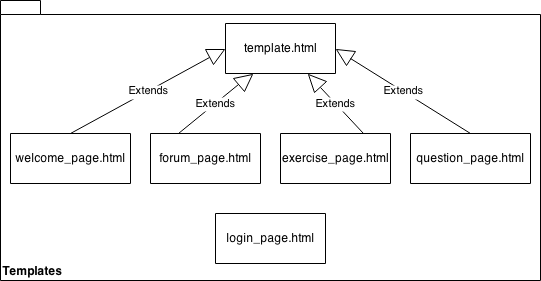
\includegraphics[width=\linewidth]{Imagens/DiagramaDeClasseTemplates.png}
    \caption{Diagrama de Classes do pacote Templates}
\end{figure}

No pacote \textbf{Views}, est\~{a}o contidos os arquivos respons\'{a}veis por tratar as
requisi\c{c}\~{o}es realizadas pelos usu\'{a}rios do sistema.

\begin{figure}[H]
    \centering
    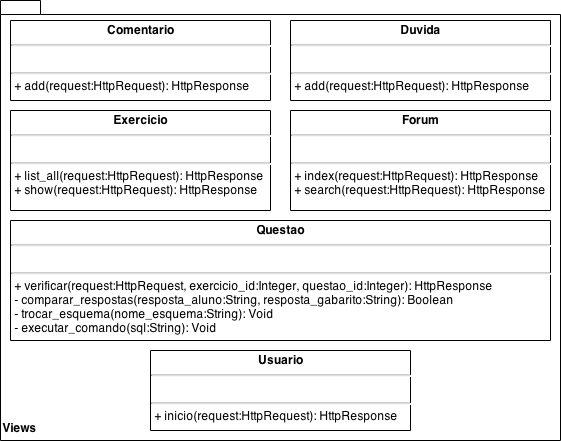
\includegraphics[width=\linewidth]{Imagens/DiagramaDeClasseViews.png}
    \caption{Diagrama de Classes do pacote Views}
\end{figure}

No pacote \textbf{Models}, est\~{a}o contidos os arquivos que servem de mapeamento objeto
relacional. Ou seja, uma representa\c{c}\~{a}o dos elementos do banco de dados.

Diferentemente das modelagens anteriores, a ilustra\c{c}\~{a}o contempla uma solu\c{c}\~{a}o
unificada entre \textbf{F\'{o}rum} e \textbf{Exerc\'{i}cios}. A figura segue na p\'{a}gina
seguinte, na horizontal, para facilitar o entendimento.

\begin{figure}[H]
    \centering
    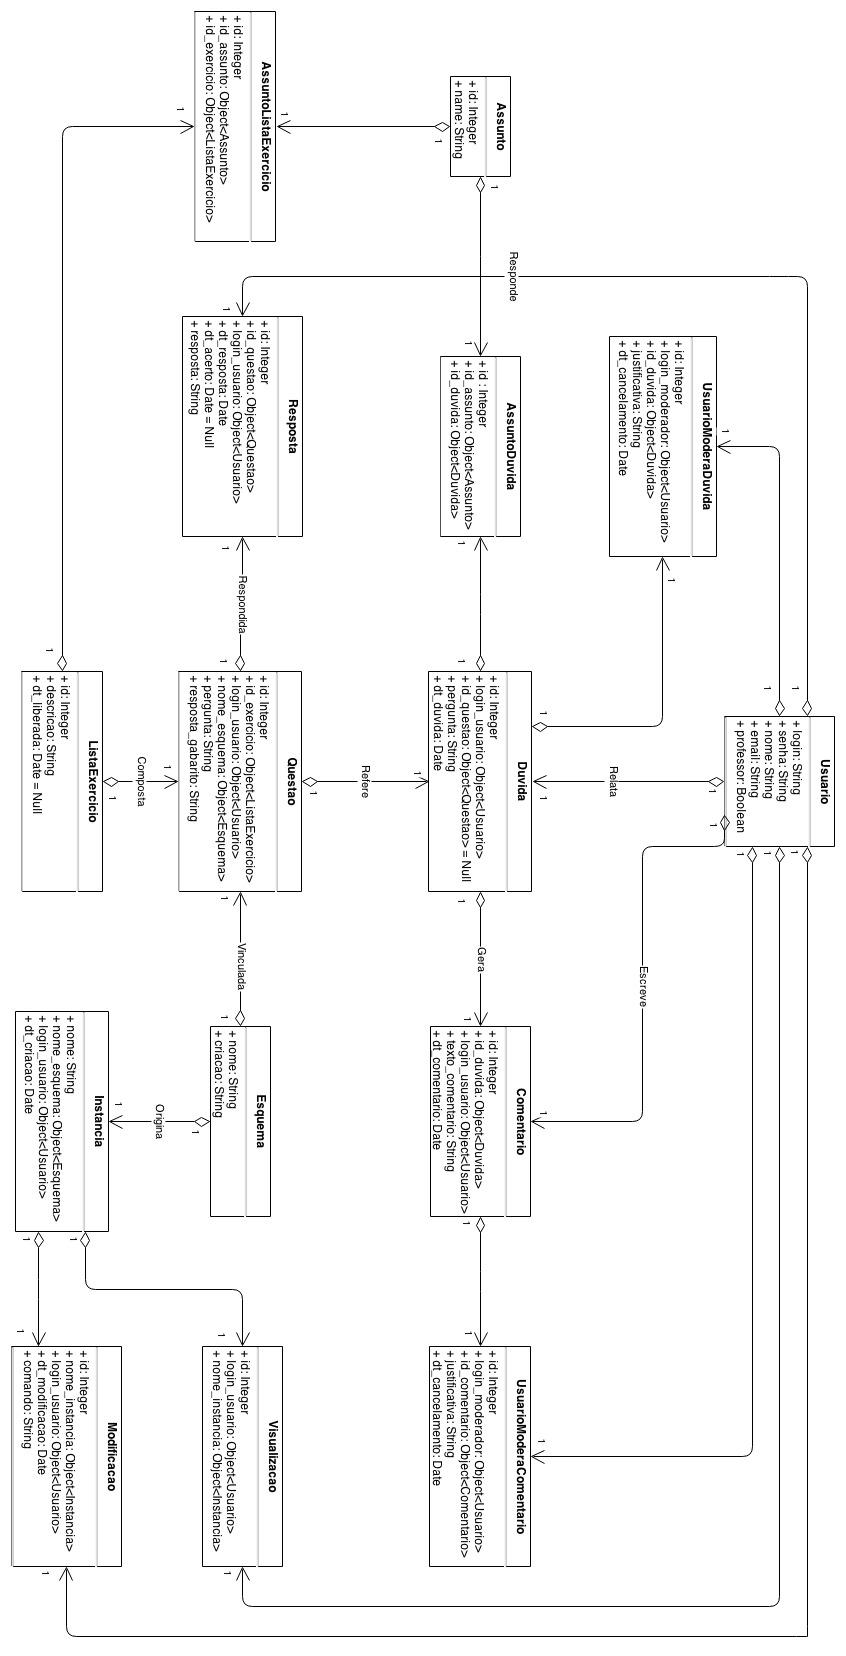
\includegraphics[width=\linewidth]{Imagens/DiagramaDeClasseModels.png}
    \caption{Diagrama de Classes do pacote Models}
\end{figure}

%%%%%%%%%%%%%%%%%%%%%%%%%%%%%%%%%%%%%%%%%%%%%%%%%%%%%%%%%%%%%%%%%%%%%%%%%%%%%%%%
% Plataforma Web %%%%%%%%%%%%%%%%%%%%%%%%%%%%%%%%%%%%%%%%%%%%%%%%%%%%%%%%%%%%%%%
%%%%%%%%%%%%%%%%%%%%%%%%%%%%%%%%%%%%%%%%%%%%%%%%%%%%%%%%%%%%%%%%%%%%%%%%%%%%%%%%

\chapter{Plataforma Web}

Este cap\'{i}tulo tem como objetivo descrever a metodologia de desenvolvimento do presente projeto,
assim como destacar todas as ferramentas utilizadas.

Como o sistema, desde seu in\'{i}cio, possui cunho opensource, foram utilizadas ferramentas do mesmo
tipo para elabora\c{c}\~{a}o do projeto. Para facilitar a documenta\c{c}\~{a}o, evolu\c{c}\~{a}o da plataforma e
acompanhamento pelo Prof. S\'{e}rgio Lifschitz, foi criado um \textbf{blog} \cite{Blog} referente ao projeto final.

Para controle de vers\~{a}o e futura participa\c{c}\~{a}o de outros interessados no projeto, foi utilizado
o \textbf{git}, atrav\'{e}s da plataforma \textbf{GitHub}. J\'{a} para organiza\c{c}\~{a}o das tarefas, fora
utilizado o \textbf{Trello}.

A fim de minimizar o tempo de desenvolvimento do sistema, optou--se por um framework para sistemas web.
O escolhido foi o \textbf{Django}, que tem \textbf{Python} como sua linguagem de programa\c{c}\~{a}o.
E, por fim, para armazenamento dos dados e aprendizado dos alunos, utilizou--se o SGBD \textbf{Postgres},
por ser gratuito, opensource e de f\'{a}cil utiliza\c{c}\~{a}o.

%%%%%%%%%%%%%%%%%%%%%%%%%%%%%%%%%%%%%%%%%%%%%%%%%%%%%%%%%%%%%%%%%%%%%%%%%%%%%%%%
% Mockups de Telas %%%%%%%%%%%%%%%%%%%%%%%%%%%%%%%%%%%%%%%%%%%%%%%%%%%%%%%%%%%%%
%%%%%%%%%%%%%%%%%%%%%%%%%%%%%%%%%%%%%%%%%%%%%%%%%%%%%%%%%%%%%%%%%%%%%%%%%%%%%%%%

\section{Mockups de Telas}

Para facilitar a etapa de desenvolvimento da plataforma, foram elaborados mocks das telas.
Dessa forma, p\^{o}de-se definir, juntamente com os \textbf{Casos de Uso} (apresentados anteriormente), como
se daria a intera\c{c}\~{a}o dos usu\'{a}rios com o sistema e o fluxo de informa\c{c}\~{a}o no
mesmo.

Seguem os prot\'{o}tipos das telas:

\begin{figure}[H]
    \centering
    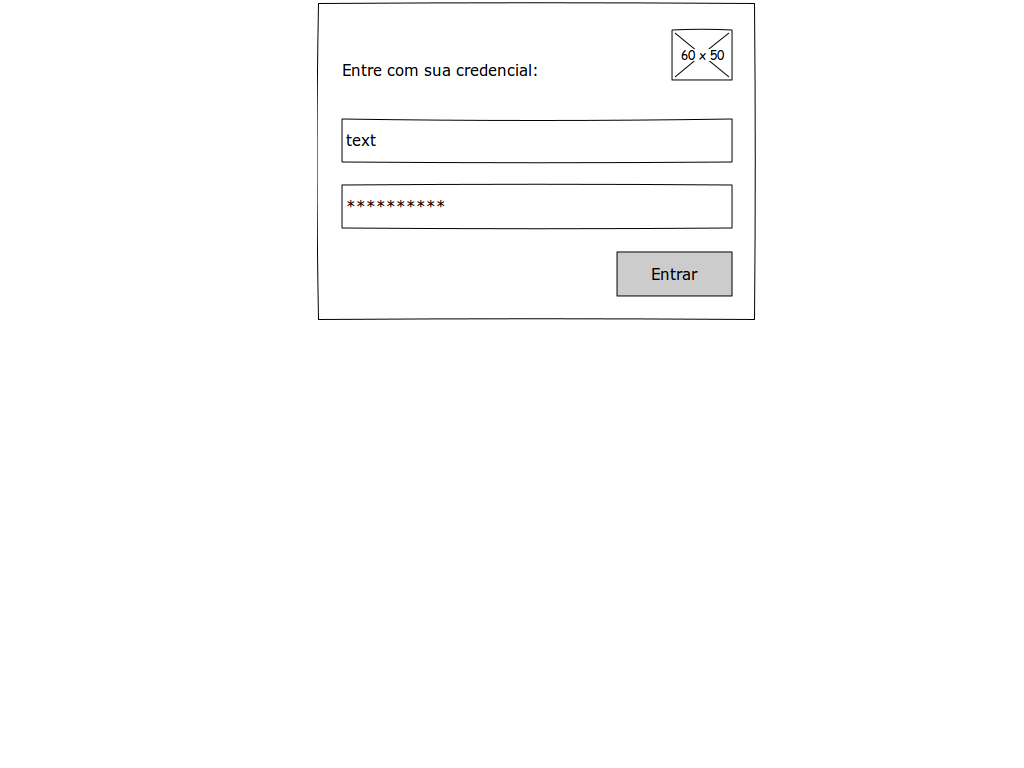
\includegraphics[width=\linewidth]{Imagens/LoginPage.png}
    \caption{P\'{a}gina para valida\c{c}\~{a}o do usu\'{a}rio}
\end{figure}

\begin{figure}[H]
    \centering
    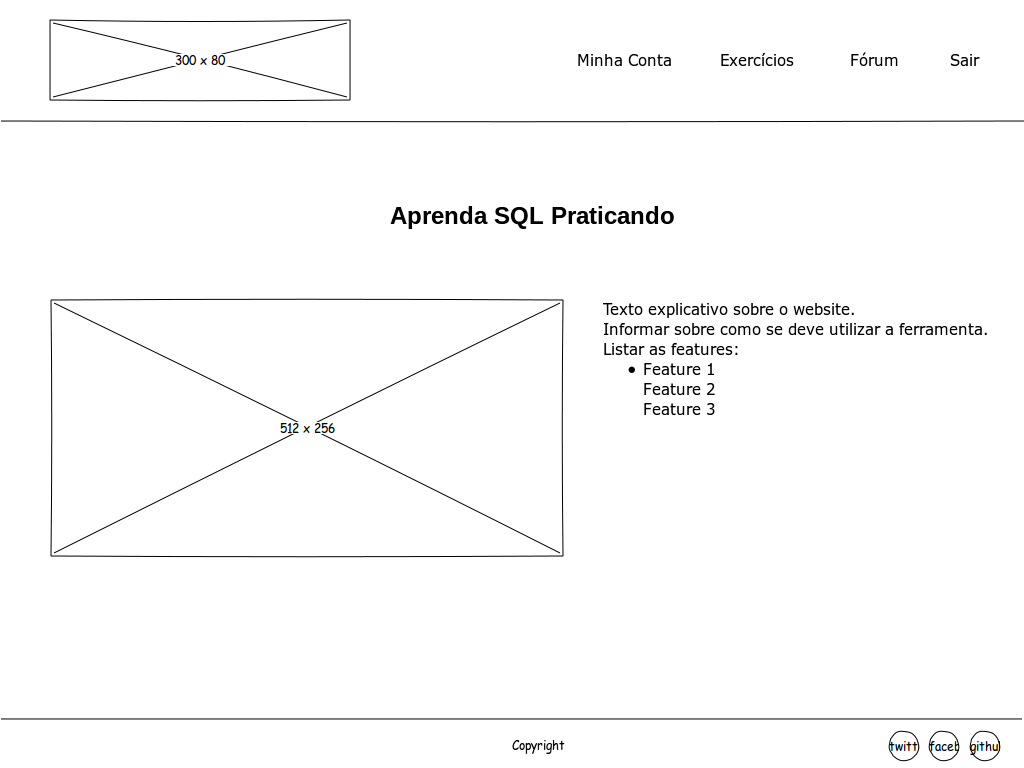
\includegraphics[width=\linewidth]{Imagens/WelcomePage.png}
    \caption{P\'{a}gina inicial do sistema}
\end{figure}

\begin{figure}[H]
    \centering
    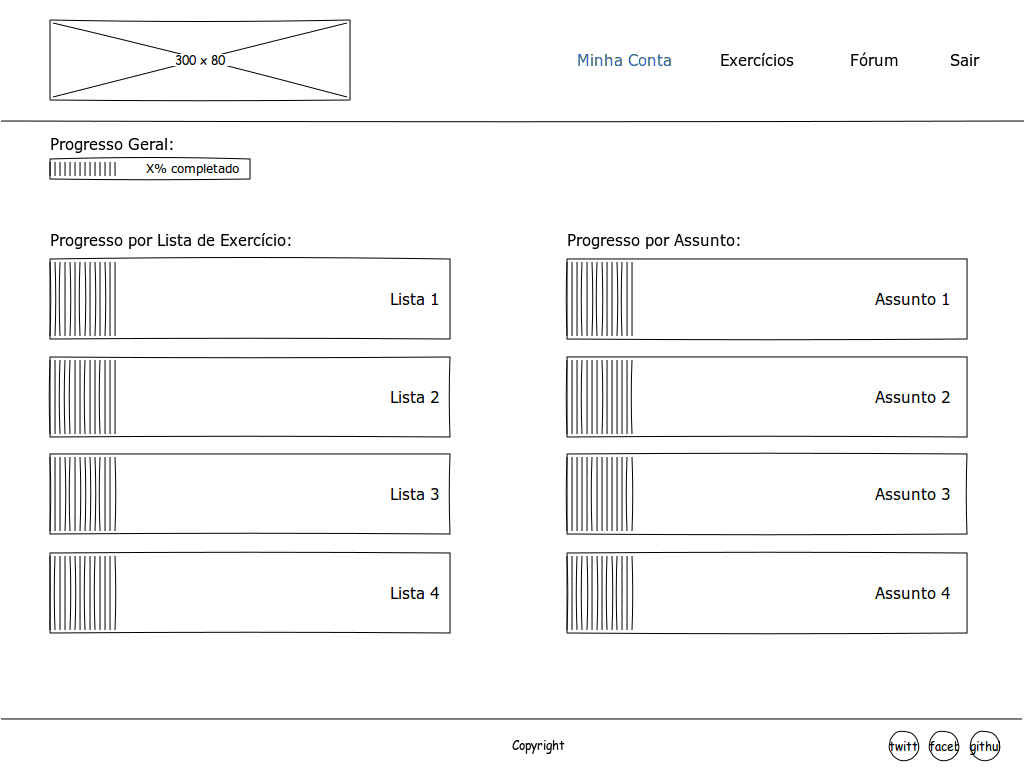
\includegraphics[width=\linewidth]{Imagens/BoardPage.png}
    \caption{P\'{a}gina que mostra o desempenho dos alunos}
\end{figure}

\begin{figure}[H]
    \centering
    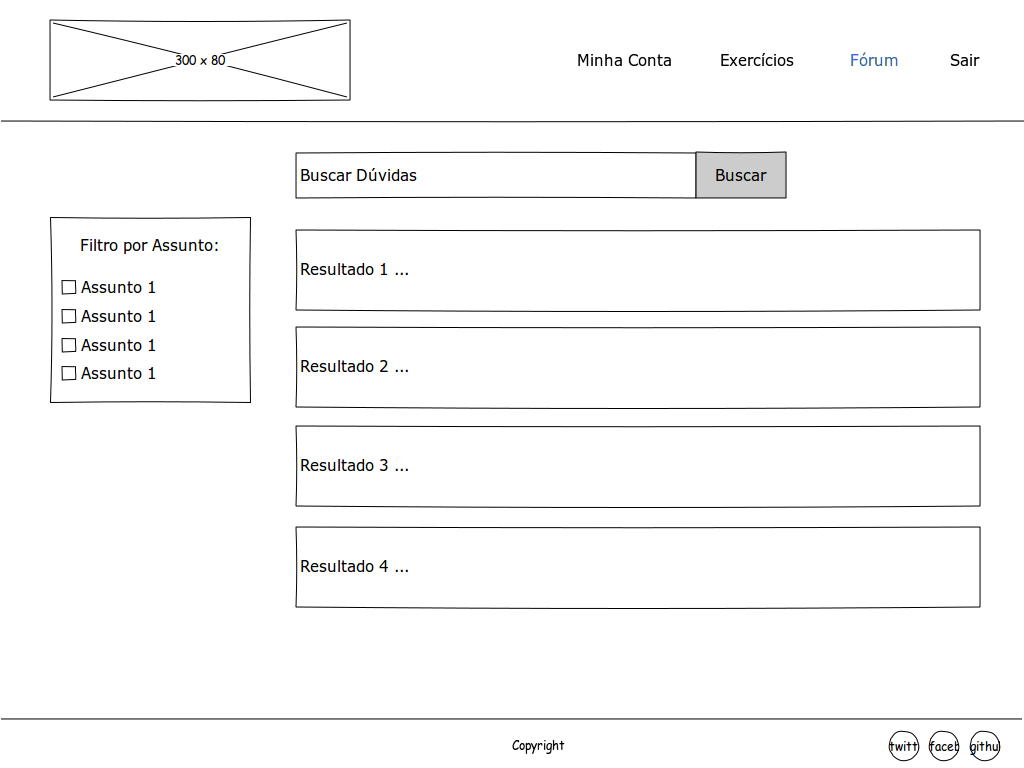
\includegraphics[width=\linewidth]{Imagens/ForumPage.png}
    \caption{P\'{a}gina de busca e inser\c{c}\~{a}o de d\'{u}vidas no f\'{o}rum}
\end{figure}

\begin{figure}[H]
    \centering
    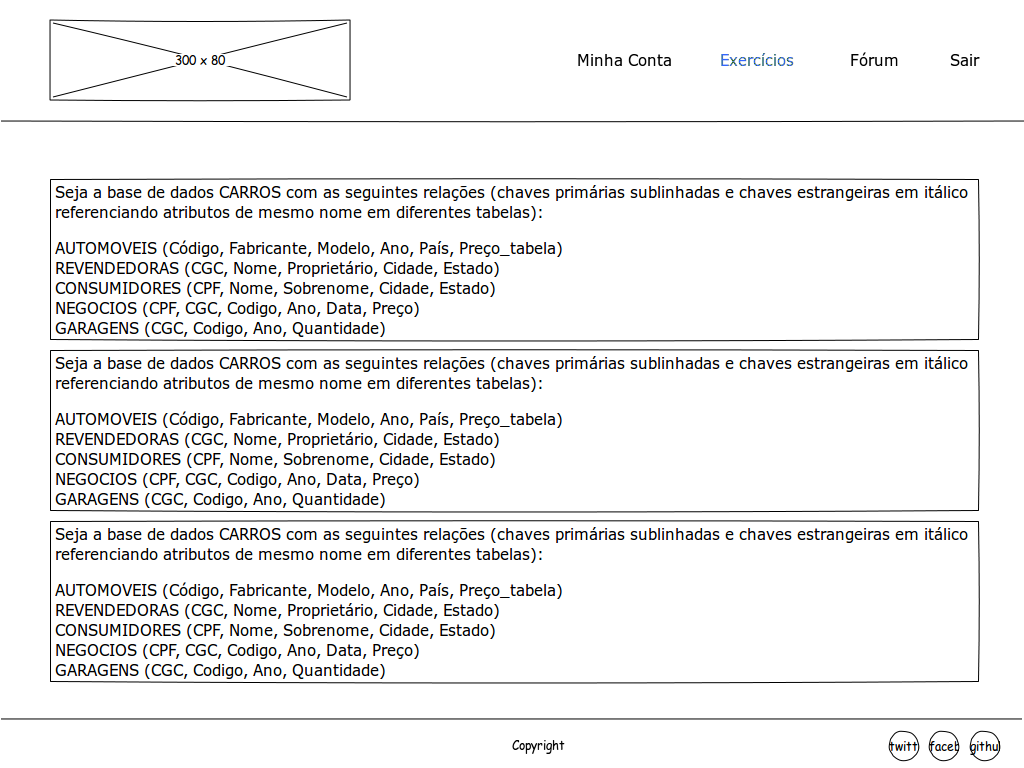
\includegraphics[width=\linewidth]{Imagens/ExercisePage.png}
    \caption{P\'{a}gina que lista os exerc\'{i}cios cadastrados}
\end{figure}

\begin{figure}[H]
    \centering
    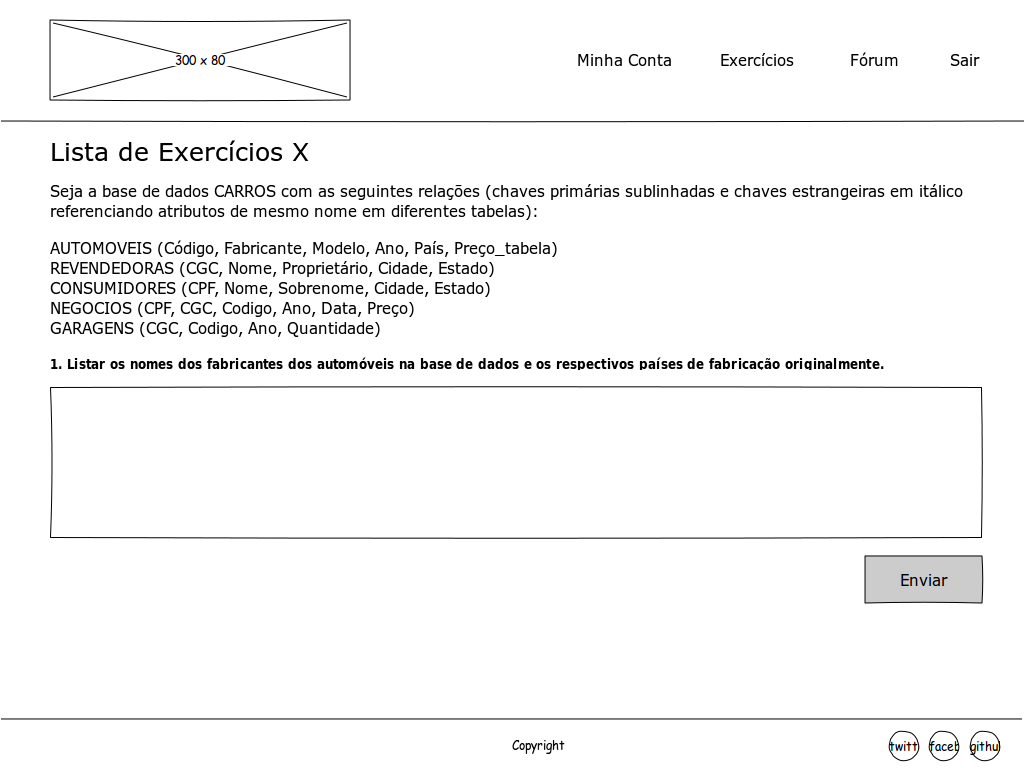
\includegraphics[width=\linewidth]{Imagens/QuestionPage.png}
    \caption{P\'{a}gina com as quest\~{o}es que comp\~{o}e a lista selecionada}
\end{figure}

\section{Framework Django}

A escolha do framework Django \cite{Django} se deu, principalmente, pela sua arquitetura bastante modularizada.
O c\'{o}digo, consequentemente, fica fortemente coeso e fracamento acoplado. Al\'{e}m disso, trata--se
de uma ferramenta que veem sendo bastante utilizada pelos desenvolvedores, o que pode facilitar
a aceita\c{c}\~{a}o da ferramenta pela comunidade de desenvolvedores.

Uma caracter\'{i}stica do framework \'{e} ser baseado na arquitetura Model--View--Template, ao inv\'{e}s
da tradicional Model--View--Controller. Por\'{e}m, ser\'{a} poss\'{i}vel perceber que trata--se apenas de
uma escolha no nome, e que, na verdade, ambas as arquiteturas s\~{a}o bastante similares.

Segue abaixo uma figura que demonstra a estrutura do framework e suas devidas explica\c{c}\~{o}es:

\begin{figure}[H]
    \centering
    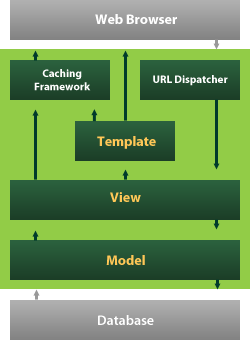
\includegraphics[width=\linewidth]{Imagens/django_structure.png}
    \caption{Arquitetura do Framework Django}
\end{figure}

\begin{enumerate}
    \item \textbf{URL Dispatcher}
    \begin{itemize}
	\item Respons\'{a}vel pelo mapeamento entre as requisi\c{c}\~{o}es feitas pelos usu\'{a}rios, baseadas na URL, 
	      e os m\'{e}todos localizados nas views, que tem por fun\c{c}\~{a}o atender \`{a}s solicita\c{c}\~{o}es.
    \end{itemize}
    \item \textbf{View}
    \begin{itemize}
	\item Respons\'{a}vel por executar as a\c{c}\~{o}es das requisi\c{c}\~{o}es realizadas, que, tipicamente,
	      envolvem leitura ou escrita no banco de dados. Pode incluir outras funcionalidades tamb\'{e}m.
    \end{itemize}
    \item \textbf{Model}
    \begin{itemize}
	\item Respons\'{a}vel pela defini\c{c}\~{a}o dos dados e a intera\c{c}\~{a}o entre os mesmos. Esse m\'{o}dulo
	      trata--se do mapeamento objeto relacional (da sigla ORM em ingl\^{e}s). Além de mapear objetos provenientes
	      do banco de dados, ele permite mapeamento em outros mecanismos de armazenamento.
    \end{itemize}
    \item \textbf{Template}
    \begin{itemize}
	\item Respons\'{a}vel pela renderiza\c{c}\~{a}o das p\'{a}ginas HTML. Permite a utiliza\c{c}\~{a}o de sintaxe
	      pr\'{o}pria, de f\'{a}cil aprendizado e similares a linguagem de express\~{a}o (da sigla UEL em ingl\^{e}s).
    \end{itemize}
\end{enumerate}

%%%%%%%%%%%%%%%%%%%%%%%%%%%%%%%%%%%%%%%%%%%%%%%%%%%%%%%%%%%%%%%%%%%%%%%%%%%%%%%%
% Considerações Finais %%%%%%%%%%%%%%%%%%%%%%%%%%%%%%%%%%%%%%%%%%%%%%%%%%%%%%%%%
%%%%%%%%%%%%%%%%%%%%%%%%%%%%%%%%%%%%%%%%%%%%%%%%%%%%%%%%%%%%%%%%%%%%%%%%%%%%%%%%

\chapter{Considera\c{c}\~{o}es Finais}

Esse trabalho teve como objetivo criar uma ferramenta online com vi\'{e}s acad\^{e}mico
e opensource, focado, inicialmente, em facilitar o ensino do conte\'{u}do da disciplina
Banco de Dados. Todas as se\c{c}\~{o}es anteriores mostraram as etapas de desenvolvimento
da plataforma, incluindo um estudo de outros softwares similares.

Atrav\'{e}s desse levantamento de dados, p\^{o}de--se perceber que a utiliza\c{c}\~{a}o 
desse aprendizado \`{a}s avessas \cite{FlippedLearning} nada mais \'{e} que uma tentativa
de aproximar os estudantes dos temas abordados em sala. Por\^{e}m, fazendo essa tentativa
de aproxima\c{c}\~{a}o via tecnologia web e mobile.

Assim sendo, teremos uma real valida\c{c}\~{a}o do projeto elaborado com a utiliza\c{c}\~{a}o
do mesmo pelos alunos nos pr\'{o}ximos per\'{i}odos seguintes. Poss\'{i}veis ajustes haver\'{a}
de serem feitos, assim como a implementa\c{c}\~{a}o de algumas funcionalidades que foram propostas,
mas n\~{a}o contempladas na presente vers\~{a}o.

Segue a lista dos requisitos que n\~{a}o foram contemplados:

\begin{itemize}
  \item [R10] Monitoramento da evolu\c{c}\~{a}o dos alunos.
  \begin{itemize}
    \item Ser\'{a} uma tela importante quando o sistema estiver em pleno funcionamento.
	  O professor da disciplina ter\'{a} possibilidade de ver um relat\'{o}rio de
	  evolu\c{c}\~{a}o da turma, em uma vis\~{a}o geral, e um relat\'{o}rio filtrando
	  por alunos.
  \end{itemize}
  \item [R11] Permiss\~{a}o para cancelar uma thread inadequada no f\'{o}rum.
  \begin{itemize}
    \item Essa funcionalidade ser\'{a} importante, pois auxiliar\'{a} a manter o f\'{o}rum
	  com temas relevantes aos dados na disciplina.
  \end{itemize}
  \item [R13] Possibilidade de compartilhar com seus colegas de turma suas inst\^{a}ncias.
  \begin{itemize}
    \item Nesta vers\~{a}o, cada aluno j\'{a} possui sua inst\^{a}ncia, a cada nova lista
	  de exerc\'{i}cios. Por\'{e}m, ainda n\~{a}o \'{e} poss\'{i}vel compartilhar suas
	  inst\^{a}ncias, assim  como n\~{a}o \'{e} poss\'{i}vel tamb\'{e}m voltar em estados
	  anteriores da mesma. Essa ser\'{a} um funcionalidade diferencial, pois permitir\'{a}
	  exerc\'{i}cios envolvendo comandos \textbf{DDL}.
  \end{itemize}
  \item [R16] Possibilidade de fazer upload de foto para facilitar a identifica\c{c}\~{a}o do aluno.
  \begin{itemize}
    \item Essa funcionalidade auxiliar\'{a}, principalmente, no acompanhamento dos relat\'{o}rios
	  por alunos, assim como no acompanhamento da participa\c{c}\~{a}o dos mesmos no f\'{o}rum.
  \end{itemize}
  \item [R17] Possibilidade de compartilhar as quest\~{o}es em redes sociais (Facebook, Google+ e Twiter).
  \begin{itemize}
    \item Apenas ser\'{a} interessante se, algum dia, a plataforma crescer e obtiver um alcance maior
	  de alunos e interessados.
  \end{itemize}
\end{itemize}

%%%%%%%%%%%%%%%%%%%%%%%%%%%%%%%%%%%%%%%%%%%%%%%%%%%%%%%%%%%%%%%%%%%%%%%%%%%%%%%%
% Bibliografia %%%%%%%%%%%%%%%%%%%%%%%%%%%%%%%%%%%%%%%%%%%%%%%%%%%%%%%%%%%%%%%%%
%%%%%%%%%%%%%%%%%%%%%%%%%%%%%%%%%%%%%%%%%%%%%%%%%%%%%%%%%%%%%%%%%%%%%%%%%%%%%%%%

\arial
\bibliography{ProjetoFinal2}

\normalfont

\end{document}